\documentclass[10pt,journal,compsoc]{IEEEtran}
%\documentclass[conference]{IEEEtran}
\IEEEoverridecommandlockouts
% The preceding line is only needed to identify funding in the first footnote. If that is unneeded, please comment it out.
\usepackage{cite}
\usepackage{amsmath,amssymb,amsfonts}
\newcommand\setItemnumber[1]{\setcounter{enumi}{\numexpr#1-1\relax}}
\usepackage{algorithmic}
\usepackage{graphicx}
\usepackage{textcomp}
\usepackage{float}
 \usepackage{url}
\usepackage{xcolor}
\def\BibTeX{{\rm B\kern-.05em{\sc i\kern-.025em b}\kern-.08em
    T\kern-.1667em\lower.7ex\hbox{E}\kern-.125emX}}
\begin{document}

\title{\textbf{Unreal Engine’s Nanite}\\ 
}


% \author{\IEEEauthorblockN{A}
% \IEEEauthorblockA{\textit{B} \\
% \textit{C}\\
% D,E \\
% F@G.com}
% \and
% \IEEEauthorblockN{H}
% \IEEEauthorblockA{\textit{I} \\
% \textit{J}\\
% K \\
% M@M.pt}
% }

%\author{\par\noindent\rule{\textwidth}{0.3pt} \\ \IEEEauthorblockN{Rui Armada}
%\IEEEauthorblockN{Universidade do Minho \\ Braga, Portugal \\ \textit{pg50737@alunos.uminho.pt}}
%\par\noindent\rule{\textwidth}{0.3pt}
%}


\author{\IEEEauthorblockN{Rui Armada} \\ Visualização em Tempo Real \\
\IEEEauthorblockN{Universidade do Minho \\ \textit{pg50737@alunos.uminho.pt}}
}


\maketitle

\IEEEpubidadjcol

\begin{abstract}
In the present document it is presented the state-of-the-art of one of Unreal Engine's latests technologies, the \textit{Unreal Engine's Nanite}. Being a new virtualized geometry technology, \textit{Nanite} is leading the gaming and entertainment industry by making it possible to create photorealistic environments with massive amount of detail and visual fidelity. Furthermore, some experimentation will be performed in order to verify if this technology is worthwhile and if it really can augment the performance of a scene.
\end{abstract}

\begin{IEEEkeywords}
Unreal Engine 5, Nanite, Virtualized Geometry, Level of Detail, Performance
\end{IEEEkeywords}

%%%%%%%%%%%%%%%%%%%%%%%%%%%%%%%%%%%%%%%%%%%%%%%%%%%%%%%%%%%
%%%%%%%%%%%%%%%%%%%%%%%%%%%%%%%%%%%%%%%%%%%%%%%%%%%%%%%%%%%

\section{Introduction}\label{sec:intro}

One of the biggest struggles of real time rendering engines, currently, is how to display a lot of detail without a big impact on the overall performance of the scene or game.

\par Usually, during the pipeline of asset development, after the construction of the high-poly version of a model, there is the need to apply optimization techniques to the asset in question. For example, surface subdivision can be used to give the viewer the idea that the model has more geometry than it actually has. The same can be said about normal mapping, usually used to “fake” bumps or even protrusions in the model, giving the illusion of texture and detail without incrementing the poly count of the model. 

\par To the untrained eye, all these techniques mentioned above offer the illusion of detail without the viewer ever noticing that, in reality, the model has a very small poly-count compared to what can be perceived. But, to the trained eye, it can be noticed some clues that are clear giveaways of the methods that were used during the asset optimization stage. For instance, in normal mapping, if the model is a sphere, and it's zoomed in immensely, the original geometry of the model can be noticed breaking the illusion that the model is fully smoothed. Furthermore, when it comes to monetary resources and time spent on the creation of the asset, it's much simpler, cheaper, and quicker to simply create a highly detailed model with a much higher polygon count; however, without proper optimization techniques, the final product will ultimately affect the performance of the actual scene being rendered. 

\par In a brief overview, Unreal Engine is one of the most popular game development engines around. It has become one of the industry standard engines for creating high-quality, interactive and immersive multimedia across various platforms. 

\par That being said, there was the need to develop a technology capable of handling assets with a high poly-count without tanking the engine's overall performance, and thus \textit{Unreal Engine's Nanite} was born. The need for a technology akin to \textit{Nanite} arose because the cost of using a different team of people to apply optimization techniques to the asset was higher than just importing the highly detailed mesh directly into the engine and using \textit{Nanite} to optimize the mesh without the labour, and time-consuming, cost attached to it.

% \par Nanite is Unreal Engine's virtualized geometry system, which uses a new internal mesh format and rendering technology to produce pixel scale detail and high object counts. It intelligently does work on only the detail that can be perceived, and no more. Nanite's data format is also highly compressed, and supports fine-grained streaming with automatic level of detail.

%%%%%%%%%%%%%%%%%%%%%%%%%%%%%%%%%%%%%%%%%%%%%%%%%%%%%%%%%%%
%%%%%%%%%%%%%%%%%%%%%%%%%%%%%%%%%%%%%%%%%%%%%%%%%%%%%%%%%%%

\section{Evolution of Real-Time Graphics}\label{sec:1}

\begin{figure}[H] 
    \centering
    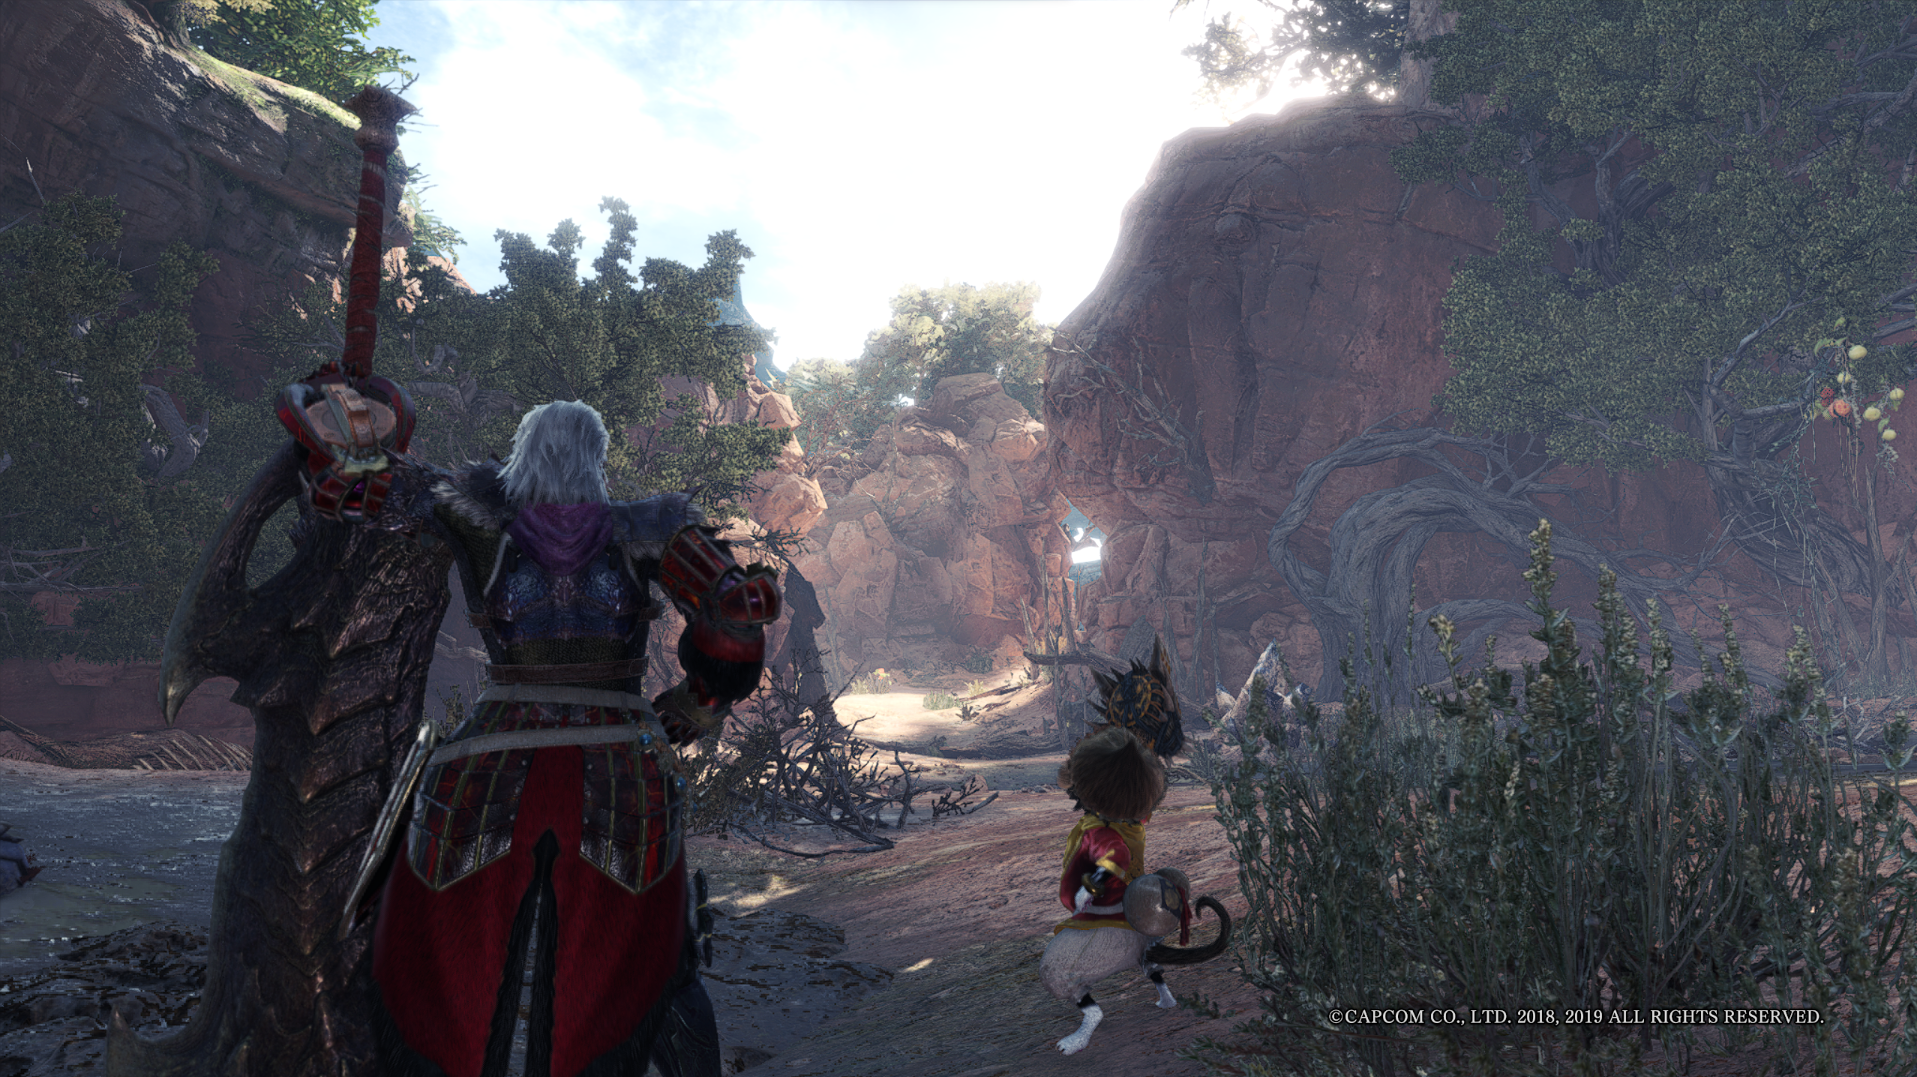
\includegraphics[scale=0.17]{img/mhw2.png}
    \caption{Capcom's Monster Hunter World was one of the games that set the bar for how to create a photorealistic, real-time 3D graphics, fantasy worlds.}
    \label{fig:mhw}
\end{figure}

\par The first edition of a 3D Game Engine Design was written in the late 1990s\cite{david} and for a long time all computer graphics remained stalled in time and looked akin to games like \textit{Tron}, \textit{Mega-Man} and even the first\textit{ Super Mario World}. At the time, all these games were a technological marvel in the 3D Graphics world but far away from the realism of the real world. Then, pre-rendered 3D started to look good enough for objects like spaceships, and now it is possible to, almost, claw all the way out of the \textit{uncanny valley} in which CG humans have often resided. So, in recent years \textit{Nvidia}, \textit{AMD} and the people interested in the CG field have been pushing the limits in order to make video games look as good as movies or other photorealistic media.

\begin{figure}[H]
    \centering
    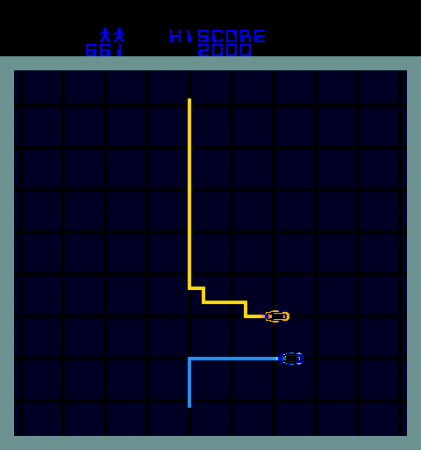
\includegraphics[scale=0.23]{img/tron.png}
    \caption{SBally Midway's Tron, released in 1982\cite{tron}.}
    \label{fig:mario}
\end{figure}

\par That being said, through the years we get closer to the objective of full immersive and photorealistic games. It's possible nowadays to write code to draw video games in engines like \textit{Unreal Engine} or \textit{Unity} to produce graphics for LED volumes that are capable and are expected to achieve photorealism. Recent releases are, occasionally, capable of producing scenes capable of provoking a fleeting impression of a real world on the other side of the display screen.

\par Until very recently, video games invariably used what was fundamentally a development of techniques going decades. First, triangles were used to make 3D objects. Why triangles? Because no matter where three points are in space, they always describe a two-dimensional flat area. At first, the triangles weren't even filled in – Wireframe graphics can be seen straight through. After this, it was concluded that the triangles would look better filled in. Then we started to attach bits of image data onto these triangles, and thus textures were born, and about the same time we started to take notice of where virtual light sources were in the scene to make the triangles brighter or darker.

\par This level of technology worked out fine through the 2000s, but there are obvious things it couldn't achieve, things that pre-rendered 3D could. Until recently, video games weren't capable of displaying accurate reflections, they could sometimes do something that looked like a reflection of the environment on a chromed out surface, but it was just a fixed image that didn't represent changes in the environment that's being reflected. They also couldn't achieve an accurate shadow system; without a lot of workarounds, usually the shadow of an unmoving object was a pre-rendered image pasted onto the triangles of the floor to simulate light and shadow.

\begin{figure}[H]
    \centering
    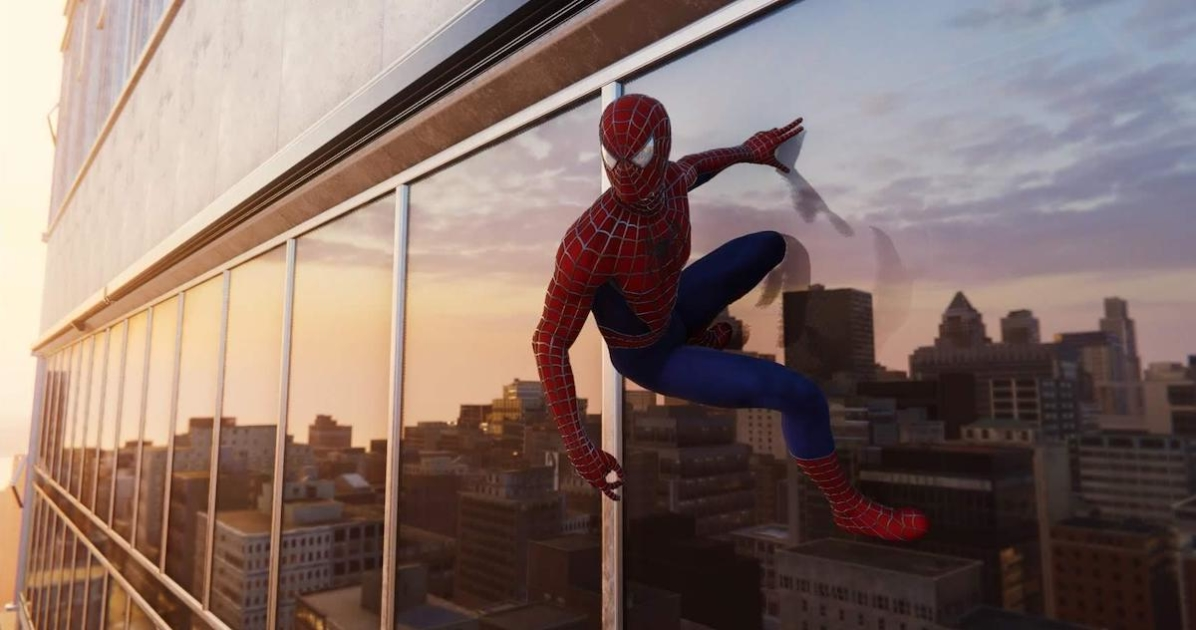
\includegraphics[scale=0.14]{img/reflection.jpg}
    \caption{Without any type of ray-tracing, the image reflected is a static image of the city to the point that it doesn't capture the character\cite{refl}.}
    \label{fig:reflect}
\end{figure}

This creates a good example of the sort of limitations real-time 3D engines often impose in order to achieve what they do. With this, there was the need to build newer technologies capable of bypassing these issues and replicating accurate images with the maximum of visual fidelity possible, and so \textit{Unreal Engine's Nanite} is one of those technologies, capable of bypassing the problem of loss of mesh detail during the process of asset optimization and producing meshes with huge amounts of detail without plummeting the engine's performance.

%%%%%%%%%%%%%%%%%%%%%%%%%%%%%%%%%%%%%%%%%%%%%%%%%%%%%%%%%%%
%%%%%%%%%%%%%%%%%%%%%%%%%%%%%%%%%%%%%%%%%%%%%%%%%%%%%%%%%%%

\section{What is Nanite?}
\label{subsec:2.1}

    \textit{Nanite} is the solution to the problem of importing assets, with immense detail, into real time rendering engines just like Unreal. For starters, \textit{Nanite} is a virtualized micropolygon\footnote{ Micropolygons are tiny polygons that represent the smallest visible details in a scene, such as individual pebbles or grains of sand.} geometry system introduced in Unreal Engine 5. It is a rendering technology that enables the rendering of extremely detailed and complex 3D environments in real-time. Furthermore, Unreal Engine's \textit{Nanite} follows the following core concepts and principles:

    \begin{itemize}
    
         \item \textbf{Detail preservation:} \textit{Nanite}'s core principle is to preserve details and fidelity in the scene to be rendered. It achieves this by dynamically adapting the level of detail based on the camera's proximity to objects. As the camera gets closer, \textit{Nanite} seamlessly loads higher-resolution micropolygons to maintain sharpness and detail, resulting in a more realistic and immersive experience.
        
        \item \textbf{Micropolygon Geometry:} \textit{Nanite} uses a micropolygon geometry system in order to render highly detailed meshes and environments. Instead of relying on traditional triangle-meshes, \textit{Nanite} breaks down geometry into tiny pieces, micropolygons, which are small surface patches that can be as small as a pixel. This approach allows for highly detailed surfaces and eliminates the need for pre-baked LODs or manual optimization of geometry.

        \item \textbf{Virtualized Geometry:} \textit{Nanite} uses a virtualized geometry approach, where only the visible portions of the geometry are loaded into memory and processed. This allows the rendering of massive environments with billions of polygons while keeping memory usage in check. It leverages virtual texturing and hardware virtual memory to efficiently stream and manage the geometry data involved in the scene.
        
        \item \textbf{Hierarchical Level of Detail (LODs):} \textit{Nanite} also incorporates a hierarchical level of detail system to manage the complexity of large scenes. It automatically generates LODs based on the level of detail required for a given area or camera distance. This helps the optimization of performance by dynamically reducing the number of polygons rendered in real-time.
        
        \item \textbf{Scalability and Performance:} \textit{Nanite} is designed to scale across different hardware configurations. It leverages modern GPU features like hardware-accelerated ray tracing and variable rate shading to deliver real-time performance, even with highly detailed scenes. \textit{Nanite} also supports other rendering features like global illumination, dynamic lighting and advanced materials to enhance overall visual quality.
    \end{itemize}

    \par In summary, \textit{Nanite} revolutionized real-time rendering by enabling the rendering of incredibly detailed and complex 3D environments. By utilizing all the core principles mentioned above, it can offer a high level of visual fidelity while maintaining real-time performance. 
    

% \begin{figure}[h]
%     \centering
%     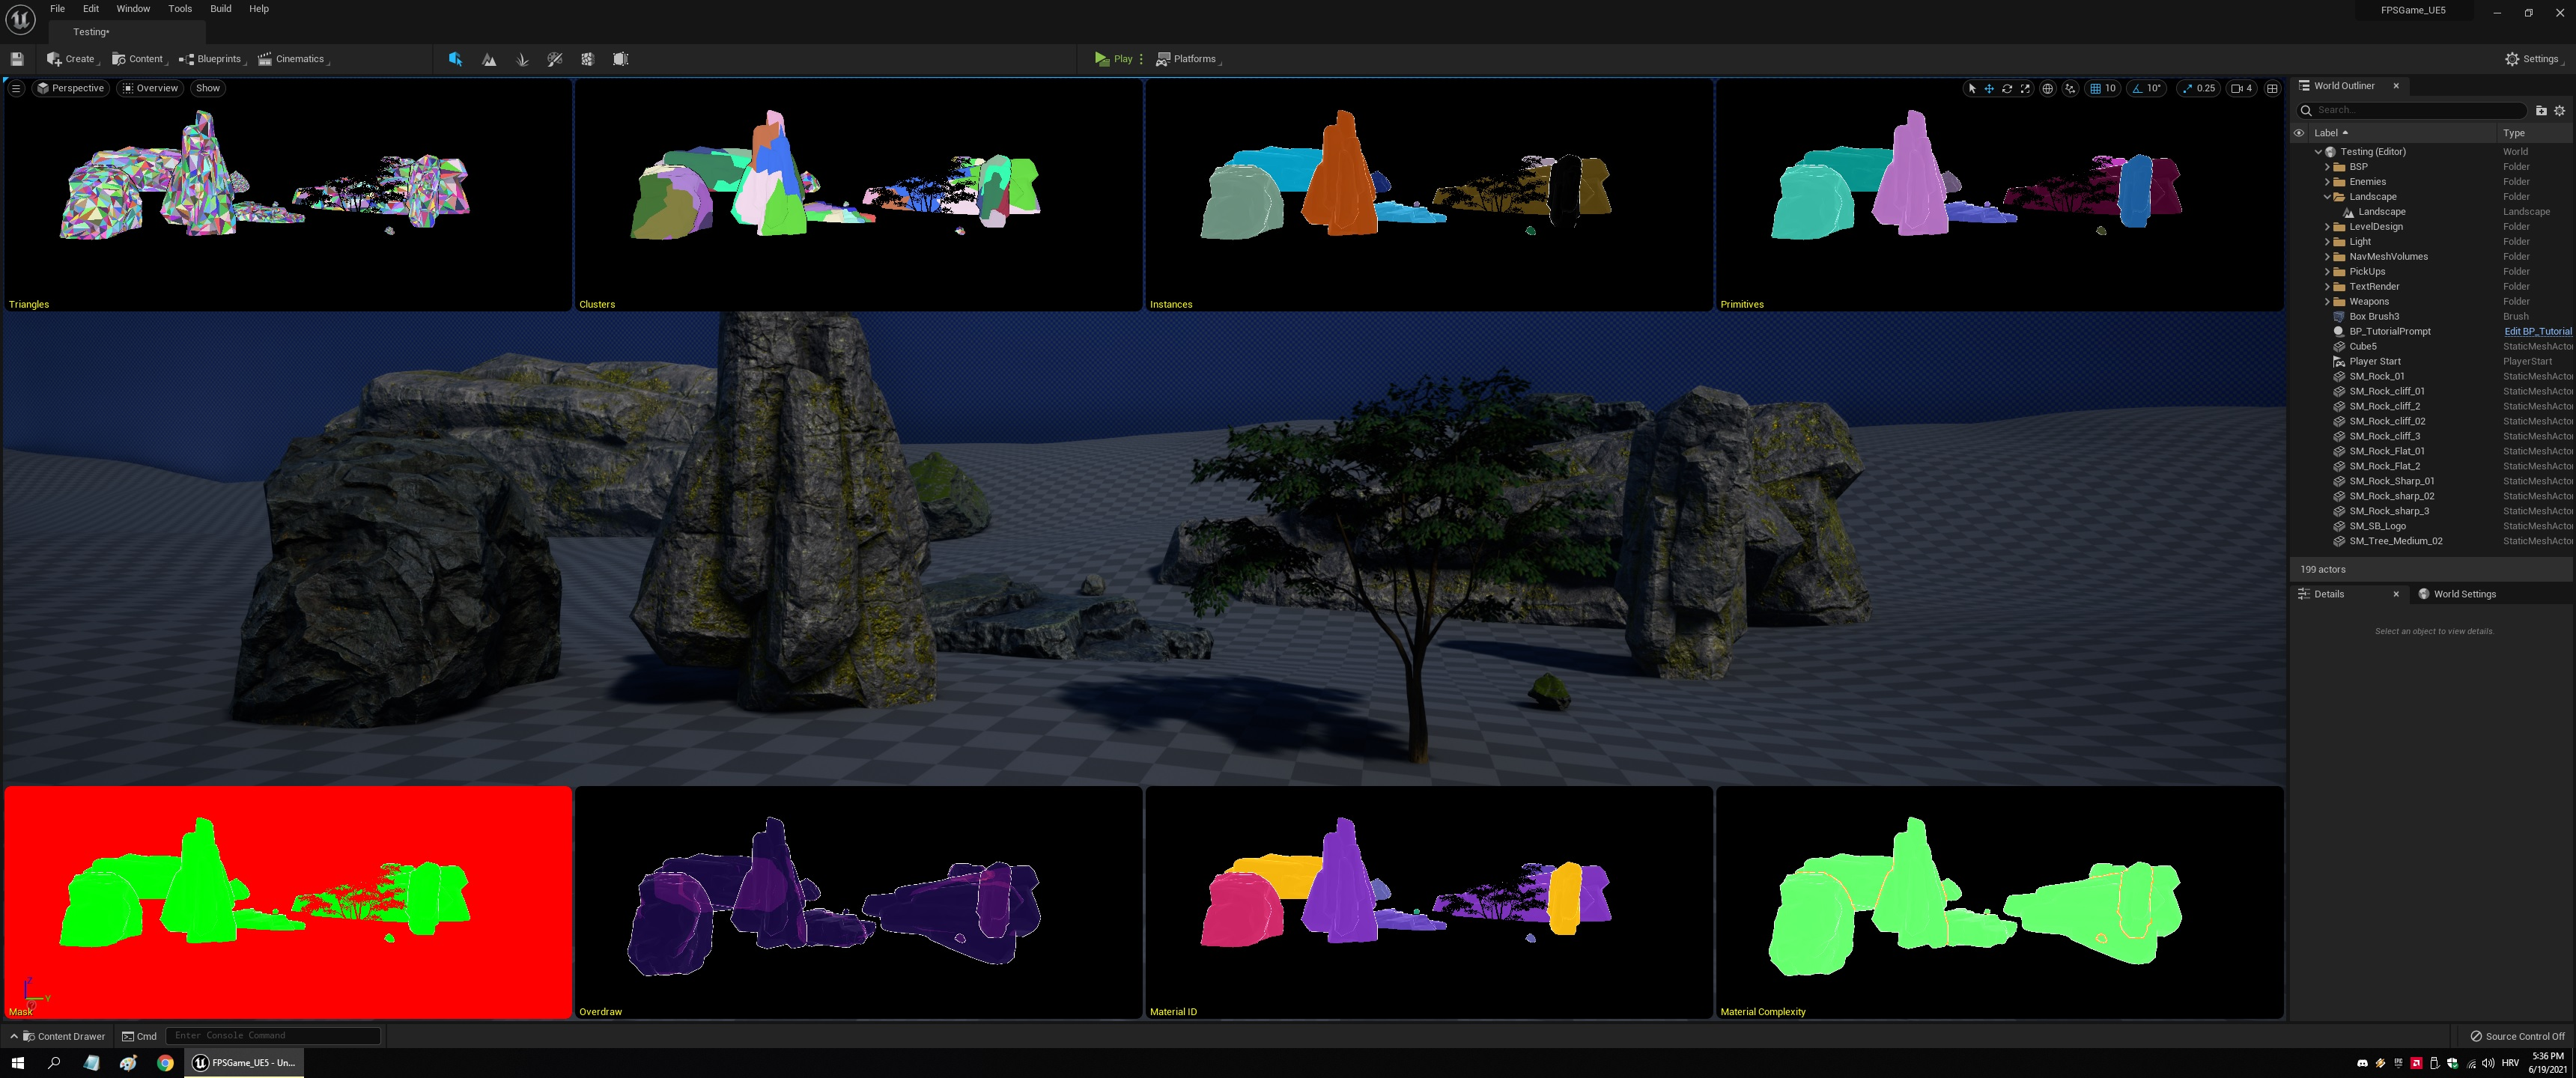
\includegraphics[scale=0.1]{img/nanite.jpg}
%     \caption{Nanite running on Unreal Engine 5.}
%     \label{fig:nanite}
% \end{figure}


%%%%%%%%%%%%%%%%%%%%%%%%%%%%%%%%%%%%%%%%%%%%%%%%%%%%%%%%%%%
%%%%%%%%%%%%%%%%%%%%%%%%%%%%%%%%%%%%%%%%%%%%%%%%%%%%%%%%%%%

% \subsection{How does Nanite work?}
% \label{subsec:2.3}

% Cross check all this
% \par In traditional real time rendering engines, geometry is stored in memory as a collection of polygons or “meshes”. The engine then uses these meshes to render the scene on the screen. However, this approach can limit the amount of detail that can be included in a scene because rendering too many polygons can be slow and impact the overall performance.

% \par Nanite, on the other hand, uses a virtualized geometry system. This means that instead of storing meshes directly in memory, the engine creates a “virtualized” representation of the geometry. This virtual representation can be divided into small, manageable chunks called “micropolygons”.

% \par These micropolygons are essentially tiny triangles that are small enough to represent individual pixels on the screen. Because of their small size, they can be rendered quickly and efficiently, even in scenes with millions of polygons. In other words, \textit{Nanite} can handle more geometry with less memory and processing power than traditional methods.

% \par  One of the key benefits of this approach is that it allows for dynamic geometry, meaning that the geometry in a scene can change in real-time without impacting performance. For instance, if a building is destroyed by an earthquake, the geometry of the building can change dynamically, and \textit{Nanite} will handle the updated geometry without any significant performance impact.

% Another advantage of \textit{Nanite} is that it supports virtual texturing, which is a technique for rendering highly detailed textures in real-time, without having to load them all into memory at once. Virtual texturing allows developers to use higher resolution textures without worrying about memory limitations.

% \textit{Nanite} also supports dynamic lighting and shadows, making it easier for developers to create realistic environments. The technology uses a new lighting model called \textit{Lumen}, which simulates indirect lighting in real-time. This approach allows for more natural lighting effects and reduces the need for precomputed lighting solutions. \textit{Lumen} will be further explained later in the document.

% \par Overall, \textit{Nanite} is a significant breakthrough in real-time rendering technology, and it has the potential to transform the way game developers create and render complex environments. The technology is currently available in early access in Unreal Engine 5\footnote{Last checked: 11 of may 2023.}, and it will likely have a significant impact on the gaming and entertainment industry going forward.

%%%%%%%%%%%%%%%%%%%%%%%%%%%%%%%%%%%%%%%%%%%%%%%%%%%%%%%%%%%
%%%%%%%%%%%%%%%%%%%%%%%%%%%%%%%%%%%%%%%%%%%%%%%%%%%%%%%%%%%

\section{Building Nanite}\label{sec:3}

\par In this section, it shall be examined all the technical and artistic aspects that enabled the creation of \textit{Nanite}. Firstly, it will be examined the artistic points that were taken into account, including the main strategies that were considered in order to build a solid foundation for this technology. Then, it will be examined the technical points and implementation of \textit{Nanite}.

% \subsection{What was considered in order to build Nanite?}\label{subsec:2.2}

\subsection{Artistic Assumptions}

\par If the geometry is virtualized, the problem of budgets for geometry would cease to exists. So, in order to build \textit{Nanite}, there was the need to take into account some strategies that would possibly help in achieving this goal. 

\par Firstly, there was the idea of using Voxels\footnote{A Voxel is a single sample, or data point, on a regularly spaced, three-dimensional grid. } in order to build this technology. A lot of considerations needed to be made about the use of voxelization to achieve a virtualized geometry system, for instance when a certain \textit{mesh} is resampled into Voxels it can look malformed. This happens because voxelization is a form of uniform resampling, and this induces loss in mesh detail and form.

\par In short, the issue with data size when voxelization is used remains too problematic in order to utilize this strategy for the virtualized geometry system. In order to replace explicit surfaces completely, many years and effort would be necessary to achieve the desired results\cite{karies_stubbe_wihlidal_00}. 

\begin{figure}[H]
    \centering
    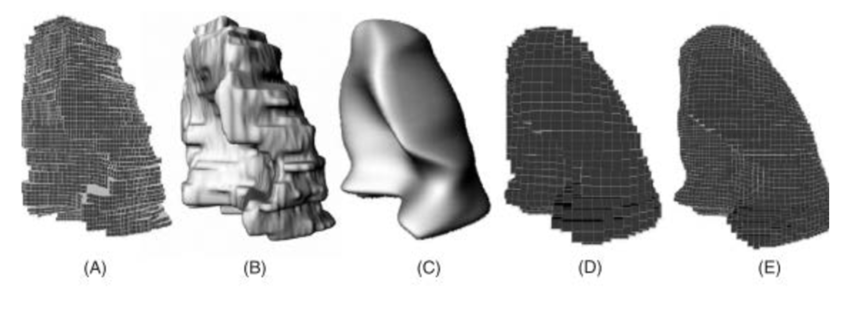
\includegraphics[scale=0.8]{img/Voxels.png}
    \caption{Voxelization example\cite{voxl}.}
    \label{fig:voxels}
\end{figure}

\par Secondly, subdivision surfaces were considered. Subdividing a surface by definition is amplification only. This method gives great results up close, but the wireframe of the mesh doesn't get more simplified than the original one. In fact, it gets more complex the more subdivided the surface is, and it gets a higher poly count than the typical game low poly meshes, which affects the performance of the renderer. More polygons instigate more memory use that affects negatively the performance, which can be seen through low fps values and incrementally high draw calls. % check this

\begin{figure}[H]
    \centering
    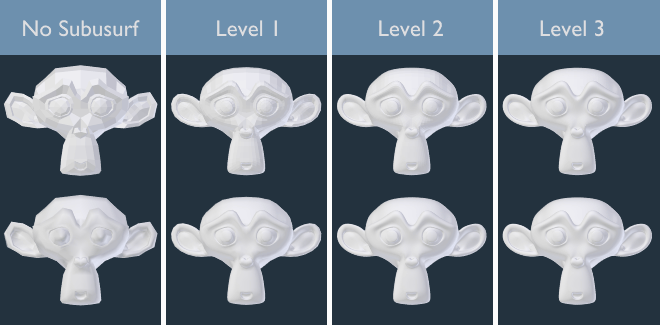
\includegraphics[scale=0.3]{img/subdivision.png}
    \caption{Subdivision levels 0 to 3, without and with Smooth Shading\cite{subdiv}.}
    \label{fig:subdivision}
\end{figure}

In addition, Displacement maps were taken into consideration. Basically, a displacement map can be viewed the same as a bump or even a normal map but far more powerful. A displacement map is, in essence, a texture map made to displace and manipulate actual geometry, meaning that shadows and silhouettes are also affected, and the lighting will also look as accurate as having handmade displacements. Naturally, this method comes with its costs: if the mesh is very basic in terms of poly count, there is no room for simple displacements because the genus of a surface can't increase. In other words, it's impossible to turn a cube into a torus using displacement mapping. It is also worth to mention that displacement mapping is a form of uniform resampling – this technique works well on organic surfaces that are already uniformly sampled, but proves really destructive on hard surfaces if not carefully controlled. It is great for up close and amplification, but not good enough for general purpose simplification.

\begin{figure}[H]
    \centering
    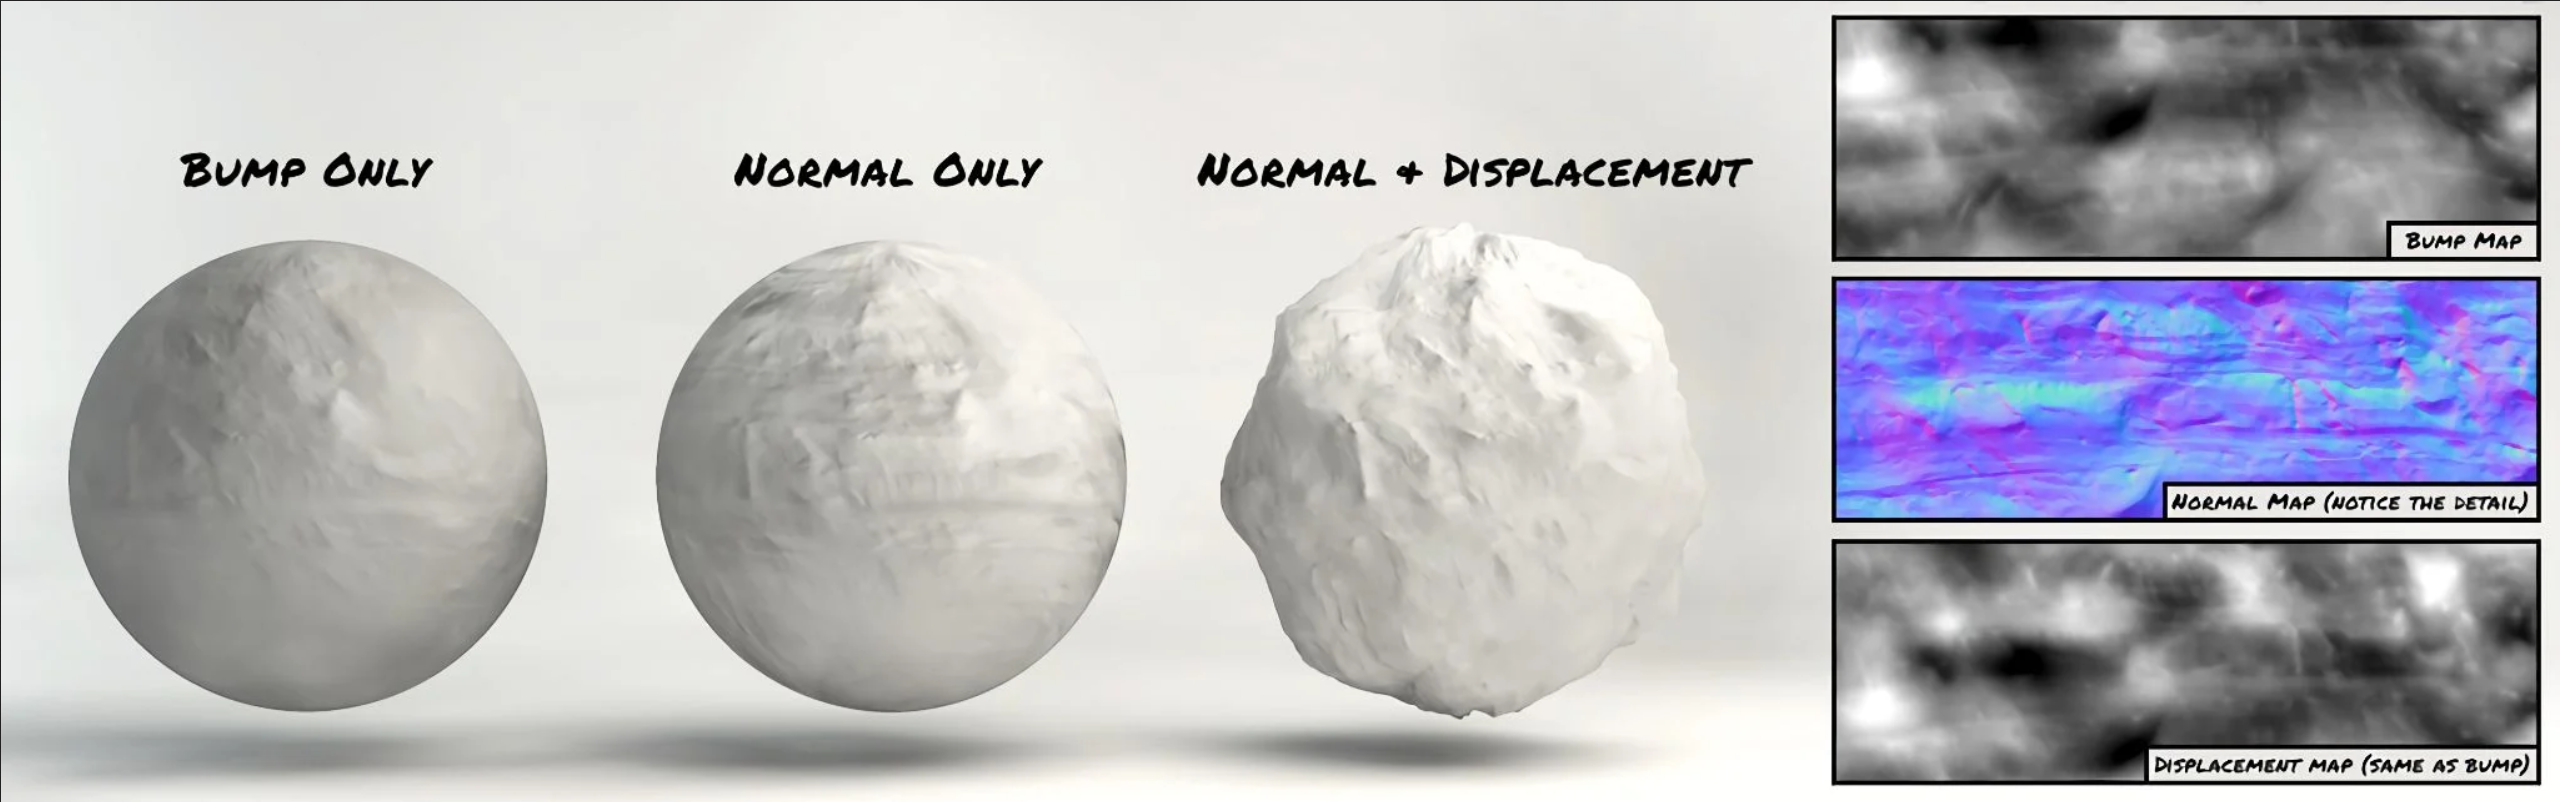
\includegraphics[scale=0.18]{img/displacement.png}
    \caption{Displacement Mapping example\cite{disp}.}
    \label{fig:displacement}
\end{figure}

After a long period of consideration, there was no faster or higher quality solution other than using triangles as the core of \textit{Nanite}. In conclusion, if it is necessary to establish an artistic style based on these other approaches, taking into account their strengths and weaknesses, they can be highly effective and yield satisfactory results, but Unreal itself \textbf{cannot dictate} an artistic style.

\subsection{Technical Assumptions}

\par It is necessary to approach the technical points of \textit{Nanite} from the perspective of requirements. In the past ten years, the development of 3A games has gradually tended to two main points: \textbf{interactive film narrative} and \textbf{open world}. In order to cutscene realistically, there is the need for exquisite character models and sufficiently flexible and rich open worlds. The map size and the number of objects have increased exponentially, both of which have greatly increased the requirements for the fineness and complexity of a scene - \textbf{usually the number of objects is much larger and each object is much more detailed}.
 
\par With this, there are usually two major bottlenecks in the rendering of complex environments:

\begin{enumerate}
    \item The CPU-side verification and communication overhead between CPU-GPU brought by each Draw Call;
    \item Overdraw caused by inaccurate elimination and the resulting waste of GPU computing resources;
\end{enumerate}

\par In recent years, the optimization technology has often revolved around these two problems, and some technical consensus in the industry has been formed.

\par In view of the overhead caused by CPU-side verification and status switching, there is now a new generation of graphics APIs\footnote{\textit{Vulkan}, \textit{DX12} and \textit{Metal}}, which are designed for the following optimizations:

\begin{itemize}
    \item Allow graphics drivers to do less verification work on the CPU side;
    \item Being able to dispatch different tasks through different Queues For GPU (Computer/Graphics/DMA Queue);
    \item Synchronization between CPU and GPU is required to be handled only by the developers;
    \item Make full use of the advantages of multicore CPU and multi-thread to submit commands to GPU;
\end{itemize}

\par Thanks to these optimizations, the number of Draw Calls of the new generation graphics API has increased by an order of magnitude compared with the previous generation graphics API\footnote{\textit{DX11}, \textit{OpenGL}.}.

\par Another optimization direction is to reduce the data communication between the CPU and GPU, and more accurately remove triangles that do not contribute to the final picture. Based on this idea, GPU Driven Pipelines were born. 

\par Thanks to the more and more widespread application of GPU driven Pipelines in games, the vertex data of a model is further divided into more fine-grained clusters\footnote{Also known as “meshlets”.} so that the granularity of each cluster can better adapt to the Vertex Processing stage. Cache size and various types of culling (\textit{Frustum Culling}, \textit{Occlusion Culling} and \textit{Backface Culling}) have gradually recognized this new vertex processing flow.

\par However, the traditional GPU Driven Pipeline relies on Compute Shader (CS) culling. The removed data needs to be stored in the GPU buffer via APIs; then, the removed Vertex/Index Buffer is fed back to the GPU's Graphics Pipeline, which has increased the invisible overhead of reading and writing. In addition, the data will be read repeatedly (CS reads before culling and the pipeline reads through Vertex Attributes when drawing).

\par Based on the previous reasons, in order to further improve the flexibility of vertex processing, Nvidia first introduced the concept of Mesh Shader, hoping to gradually remove some fixed units in the traditional vertex processing stage.

\begin{figure}[H]
    \centering
    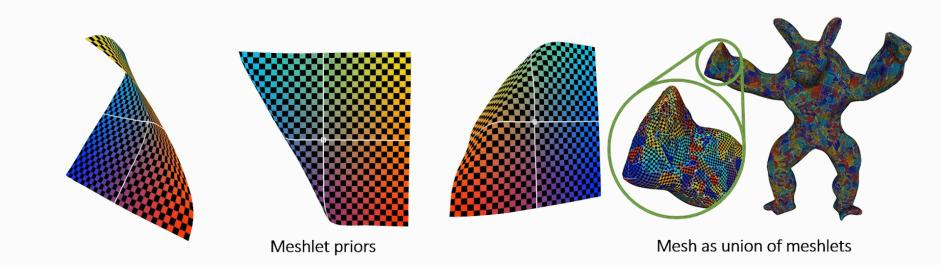
\includegraphics[scale=0.35]{img/meshlets.jpg}
    \caption{Mesh representation in Clusters/Meshlets\cite{cluster}.}
    \label{fig:meshlets}
\end{figure}

\begin{figure}[H]
    \centering
    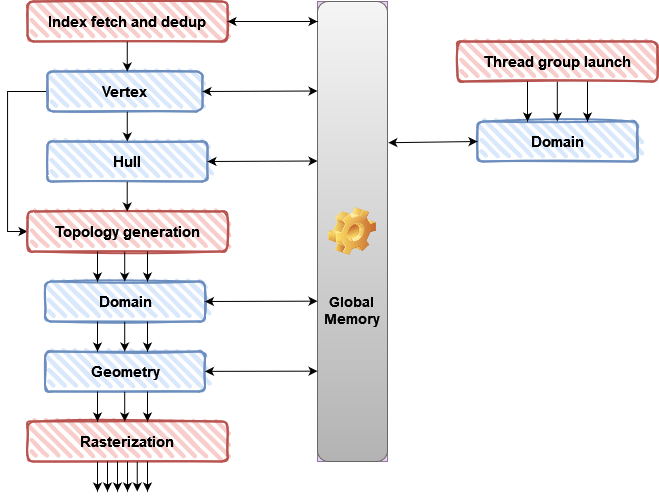
\includegraphics[scale=0.26]{img/diagram1.png}
    \caption{Traditional GPU Driven Pipeline eliminates dependence on CS, and the eliminated data is passed to the vertex processing pipeline through VRAM.}
    \label{fig:diagram1}
\end{figure}

\begin{figure}[H]
    \centering
    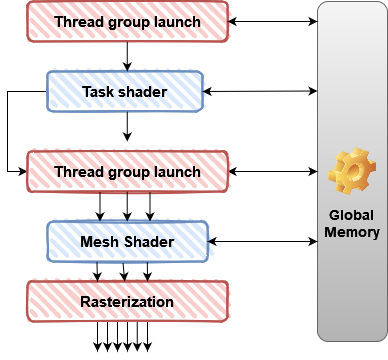
\includegraphics[scale=0.26]{img/diagram2.png}
    \caption{Pipeline Based on the Mesh Shader, Cluster culling becomes part of the vertex processing stage, reducing unnecessary Vertex Buffer Load/Store.}
    \label{fig:diagram12}
\end{figure}

% \subsection{Are these enough?}

% \par So far, the problems of the number of models, the number of triangle vertices and the number of faces have been greatly optimized and improved. However, high-precision models and small triangles at pixel lever put new pressure on the rendering pipeline: \textbf{Rasterization} and \textbf{Overdraw pressure}.

\subsubsection{Soft Rasterization vs Hard Rasterization}\label{sec:rast}

\par In order to clarify this issue, it is imperative to comprehend the fundamental functions of hard rasterization and the broad application scenarios it envisages. To put it simply: \textbf{At the beginning of the design of traditional rasterization hardware, the size of the input triangle envisaged is much larger than one pixel}. Based on this assumption, the process of hardware rasterization is usually hierarchical.

\par Taking the Nvidia Rasterizer as an example, a triangle usually undergoes two stages of rasterization: \textit{Coarse Raster} and \textit{Fine Raster}. The former takes a triangle as input and $8\times8$ pixels as a block, and the triangle is rasterized into several blocks. 

\par At this stage, the occluded block will be completely eliminated through the low-resolution \texttt{Z-Buffer} which is called \textbf{\textit{Z Cull}} on the Nvidia card. After the \textit{Coarse Raster}, the block that passes through the \textit{Z Cull} will be sent to \textit{Fine Raster}, which finally generates pixels for shading. In the \textit{Fine Raster} stage, begins the familiarity with \textbf{\textit{\textit{Early Z}}}. Due to calculation needs of Mip-Map sampling, the information of the adjacent pixels of each pixel must be known. The difference of the sampled UV must be used as the calculation basis for the Mip-Map sampling level. For this reason, the final output of \textit{Fine Raster} is not a pixel, but a small $2\times2$ \textbf{Pixel Quad}.

\par For triangles close to the pixel size, the waste of hardware rasterization is obvious. Firstly, the \textit{Coarse Raster} stage is almost useless, since these triangles are usually smaller than $8\times8$. This situation is even worse for the long and narrow triangles, not only because a triangle often spans multiple blocks and cannot be removed by \textit{Coarse Raster}, but also because it adds additional computational burden. Furthermore, for larger triangles, the \textit{Fine Raster} stage based on Pixel Quad will only generate a small number of useless pixels on the edge of the triangle, which is only a small part of the area of the entire triangle. However, for small triangles, pixel quad will generate pixels four times the area of the triangle at worst.

\begin{figure}[H]
    \centering
    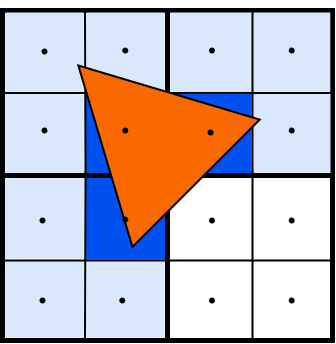
\includegraphics[scale=0.25]{img/PixelQuad.png}
    \caption{Rasterization waste of small triangles due to pixel quad.}
    \label{fig:pixelQuad}
\end{figure}

\par For these reasons, soft rasterization based on Compute Shader does have a chance to overthrow hard rasterization under the specific premise of pixel-level small triangles.

\subsubsection{Deferred Material}

\par In the evolution of the rendering pipeline, some researchers have proposed \textit{Z-Prepass}, \textit{Deferred Rendering}, \textit{Tile Based Rendering}, and \textit{Clustered Rendering} to solve the problem of redrawing. These different rendering pipeline frameworks that are used to answer the same question: \textbf{When a light source exceeds a certain value and the complexity of the material increases, how to avoid numerous rendering logic branches in the Shader and reduce redrawing?}

\par Generally speaking, the deferred rendering pipeline needs a set of \textit{Render Targets} called \textbf{\textit{G-Buffers}}. These textures store all the material information needed for lighting calculations. In today's 3A games, the types of materials are often complex and changeable, and the \textit{G-Buffer} information that needs to be stored is increasing year by year. 

\begin{figure}[H]
    \centering
    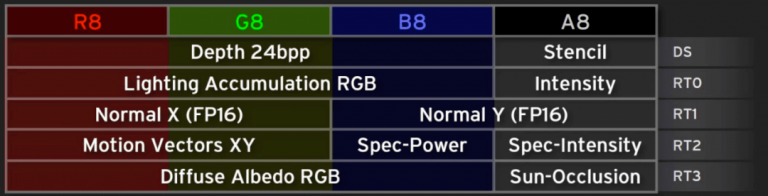
\includegraphics[scale=0.25]{img/gbuffer.png}
    \caption{Guerrilla's \textit{Killzone} 2 \textit{G-Buffer} layout.\cite{killzone}}
    \label{fig:gbuffer1}
\end{figure}

\par Excluding \textit{Lighting Buffer}, in fact, the number for \textit{G-Buffer} is 4, totalling 16 Bytes/Pixel. 

\par On the other hand, in recent years \textbf{due to the increased material complexity and fidelity, the bandwidth required by the G-Buffer has been doubled}.

\par For scenes with high Overdraw, the read and write bandwidth generated by the drawing of \textit{G-Buffer} will overcome a performance bottleneck. With this, a new rendering pipeline was introduced: the \textbf{\textit{Visibility Buffer}}. Algorithms based on \textit{Visibility Buffer} no longer generate bloated \textit{G-Buffers} alone, but instead use \textit{Visibility Buffers} with lower bandwidth overhead. The \textit{Visibility Buffer} usually needs the following information:

\begin{enumerate}
    \item \textbf{Instance ID}, which indicates which Instance ($16\approx24$ bits) the current pixel belongs to;
    \item \textbf{Primitive ID}, which indicates which triangle ($8\approx16$ bits) of Instance the current pixel belongs to;
    \item \textbf{Barycentric Coord}, which represents the position of the current pixel in the triangle, expressed in barycentric coordinates ($16$ bits);
    \item \textbf{Depth Buffer}, which represents the depth of the current pixel ($16\approx24$ bits);
    \item \textbf{Material ID}, which indicates which material the current pixel belongs to ($8\approx16$ bits);
\end{enumerate}

\par It is only needed to store about $8\approx12$ Bytes/Pixel to represent the material information of all geometries in the scene. At the same time, a global vertex and texture map must be maintained. The table stores the vertex data of all geometries in the current frame, as well as material parameters and textures.

\par In the lighting shading stage, it's only needed to index to the relevant triangle information from the global \textit{Vertex Buffer} according to the Instance ID and Primitive ID. Furthermore, according to the centre of gravity coordinates of the pixel, the vertex information in the \textit{Vertex Buffer} (UV, Tangent Space, etc.) performs interpolations to obtain pixel-by-pixel information. In addition, according to the Material ID to index the relevant material information, the \textit{Vertex Buffer} performs operations such as texture sampling and input to the lighting calculation link to complete the colouring. This type of method is sometimes called \textbf{Deferred Texturing}.

\begin{figure}[H]
    \centering
    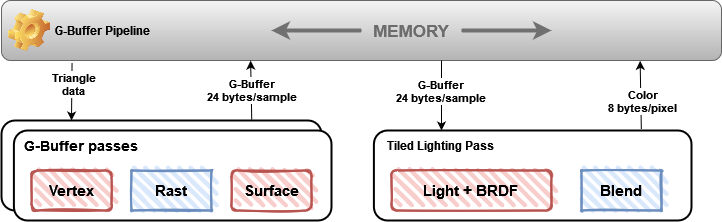
\includegraphics[scale=0.25]{img/pl1.png}
    \caption{Rendering pipeline based on \textit{G-Buffer}.}
    \label{fig:pl1}
\end{figure}

\begin{figure}[H]
    \centering
    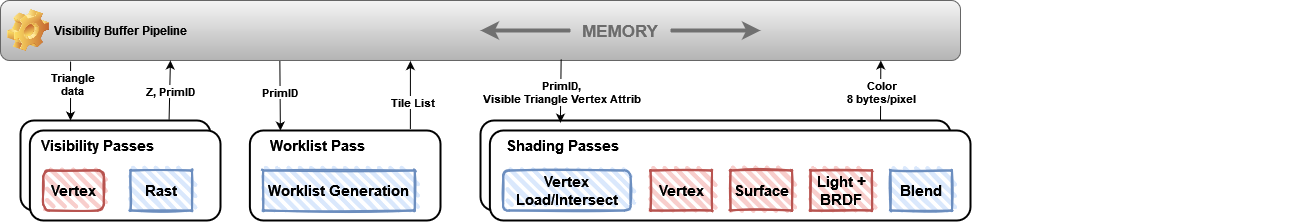
\includegraphics[scale=0.25]{img/pl2.png}
    \caption{Rendering pipeline based on \textit{Visibility Buffer}.}
    \label{fig:pl2}
\end{figure}

Intuitively, the \textit{Visibility Buffer} reduces the storage bandwidth of the information needed for shading. In addition, it delays the reading of geometric information and texture information related to lighting calculations to the shading stage, so those non-visible pixels on the screen do not need to read this data, but only need to read the vertex position. For these two reasons, \textbf{the \textit{Visibility Buffer} bandwidth overhead is greatly reduced compared to traditional \textit{G-Buffer} in complex scenes with higher resolution}. However, maintaining global geometry and material data at the same time increases the complexity of engine design and reduces the flexibility of the material system\footnote{To solve this it's possible to use certain Graphics APIs but some of them are yet not supported by all hardware.}.

\subsection{Implementation}

\par So, with the diverse array of papers, presentations, and documentation about \textit{Nanite} it's possible to deduce the way it was implemented. In addition, a good foundation about the concepts and ideas that led to this technology was necessary, and so the previous sections offer a good insight on the subject. With this, \textit{Nanite} at its core can be simply disassembled in two parts:

\begin{enumerate}
    \item Optimization of vertex processing and optimization of pixel processing. The optimization of vertex processing is mainly based on the idea of GPU Drivel Pipeline; 
    \item Optimization of pixel processing with the help of \textit{Visibility Buffer} combined with soft rasterization;
\end{enumerate}

% \textbf{METER FULL ALGORITMO - Fazer diagrama}

\subsubsection{Instance Cull \& Persistent Cull}

\par In \textit{Nanite}, each \textit{Nanite Mesh} is cut into several Clusters in the preprocessing stage. Each cluster contains 128 triangles and the entire Mesh is organized into a tree structure in \textbf{Bounding Volume Hierarchy (BVH)} and each leaf node represents a cluster of triangles. After this, there are two steps of culling, including \textit{frustum culling} and \textit{occlusion culling} based on \textbf{Hierarchical Depth Buffer (HZB)}. Among them, there are two prevalent types of culling that \textit{Nanite} uses: \textbf{Instance culling} and \textbf{Occlusion culling}.

\par \textbf{Instance culling} is one of the first things that happens in the at this stage of \textit{Nanite}. It seems akin to a GPU form of \textit{frustum} and \textit{occlusion culling}. There is an instance of data and primitive data that is bound at this stage, this means that \textit{Nanite} culls at the instance level first, and if the instance survives it starts culling at a finer-grained level, in this case the instances are the root nodes of the BVH tree of each Mesh. In addition, the \texttt{Nanite.Views} buffer provides camera info for \textit{frustum culling} and the HZB is used for \textit{occlusion culling}. With this, the HZB is generated in the current frame with the previous frame's visible objects\cite{karies_stubbe_wihlidal_0}. The HZB is tested with the previous objects as well as anything new, and the visibility is updated for the next frame.

\par Both visible and non-visible instances are written into buffers. For the latter, it's needed to inform the CPU that a certain entity is occluded, and it should stop the processing until it becomes visible. The visible instances are also written out into a list of candidates.

\par The \textbf{Persistent culling} seems to be related to streaming. It is a fixed number of compute threads, suggesting it is unrelated to the complexity of the scene and instead checks some spatial structure of occlusion. In this stage, each mesh will be sent the root node of its BVH for the hierarchical elimination of the \textit{Persistent culling} through the \textit{Instance culling}. If a BVH node is eliminated its child nodes will not be processed.

\subsubsection{Rasterization}

\par After the culling stage, each cluster will be sent to different rasterizers, mentioned in subsection \ref{sec:rast}.  In \textit{Nanite}, large triangles and non-Nanite Meshes are still based on hardware rasterization, and small triangles are based on soft rasterization written by compute shaders. \textit{Nanite's Visibility buffer} is, in essence, a texture ($8$ Bytes/Pixel) that stores two distinct channels, each with a size of $32$ bits. These channels store the following information:

\begin{enumerate}
    \item Triangle ID, $0\approx6$ bits of the R channel;
    \item Cluster ID, $7\approx31$ bits of the R channel;
    \item Depth, $32$ bits of the G channel;
\end{enumerate}

\begin{figure}[H]
    \centering
    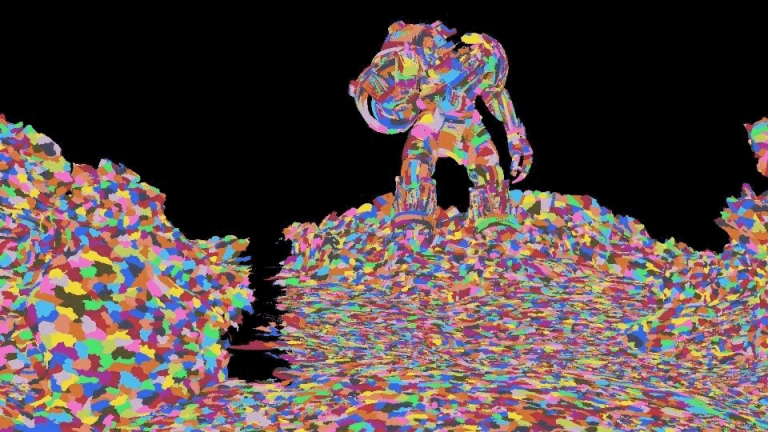
\includegraphics[scale=0.3]{img/culsterID.png}
    \caption{Cluster ID channel is one of the information textures contained in the \textit{Visibility Buffer}\cite{IGN}.}
    \label{fig:cid}
\end{figure}

\par With this, the entire logic of the \textit{soft} rasterization becomes clear.

\begin{enumerate}
    \item Based on the scan line algorithm, each cluster starts a separate Compute Shader, calculates and caches all Clip Space Vertex positions to shared memory in the initial stage of the Compute Shader;
    \item Each thread in the Compute Shader reads the corresponding Index Buffer of the triangle and the transformed Vertex Position; 
    \item The side of the triangle is calculated according to the Vertex Position;
    \item Backside elimination and small triangle culling is performed;
    \item Utilization of atomic operations to complete the \texttt{Z-Test}, and write the data into the \textit{Visibility Buffer};
\end{enumerate}

\par It's also worth mentioning that, in order to ensure that the entire \textit{soft rasterization} logic is concise, the Mesh \textbf{cannot have} any kind of deformation or skeletal animation.
 
\subsubsection{Emit Targets}

\par In order to ensure that the data structure is as compact as possible as well as reduce the read and write bandwidth, all the data required for \textit{soft rasterization} is stored in a \textit{Visibility Buffer} in order to mix the pixels generated by hardware rasterization on a scene. With this, it's finally needed to write the additional information within the \textit{Visibility Buffer} into the unified \textit{Depth/Stencil Buffer} and \textit{Motion Vector Buffer}. So, in this stage, there are several passes applied to the screen:

\begin{enumerate}
    \item \textbf{Scene Depth/Stencil, Nanite Mask and Velocity Buffer}: This phase outputs three important quantities: \underline{Depth}, \underline{Motion Vectors} and \underline{Nanite Mask}. The first two are standard quantities that are later used for things like TAA, reflections, etc. On the other hand, the \textit{Nanite Mask} is used to indicate whether the current pixel is a Normal Mesh or a \textit{Nanite Mesh}.
\end{enumerate} 

\begin{figure}[H]
    \centering
    
\includegraphics[scale=0.26]{img/NM.png}
    \caption{Nanite Mask\cite{IGN}.}
    \label{fig:dbf}
\end{figure}

\begin{enumerate}
    \setItemnumber{2}
    \item \textbf{Material Depth}: This is essentially a \textit{Material ID} turned into a unique depth value and stored in a depth-stencil target. Effectively, there is one shade of grey per material. This is going to be used next as an optimization that takes advantage of \textit{Early Z}.
\end{enumerate}

\begin{figure}[H]
    \centering
    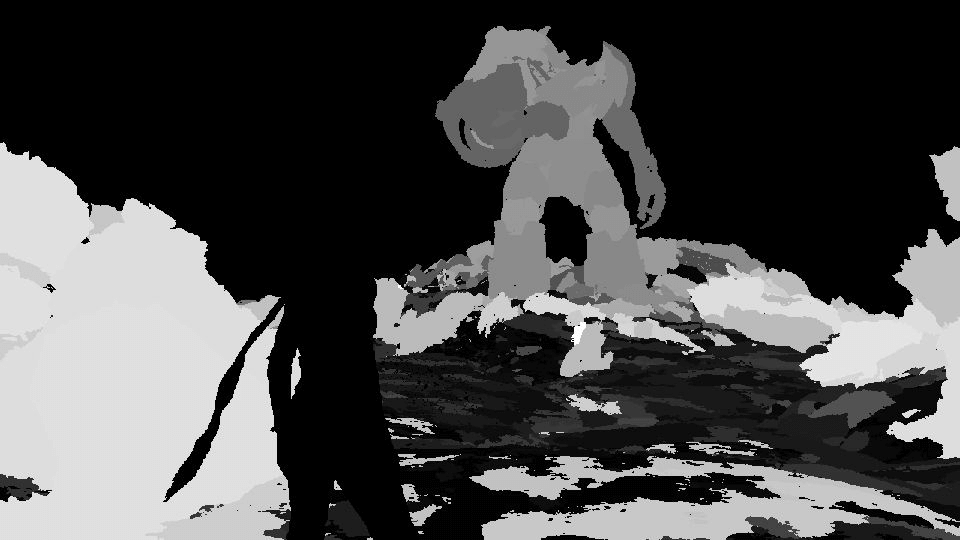
\includegraphics[scale=0.26]{img/MDB.png}
    \caption{Material Depth Buffer\cite{IGN}.}
    \label{fig:mdb}
\end{figure}

\subsubsection{Classify Materials \& Emit G-Buffer}

\par Now that the geometry pipeline has been explained in detail, it's time to talk about materials. Up until the \textit{Visibility Buffer} generation and now, the frame spends a great amount of runtime doing other tasks: light grid, sky atmosphere, and rendering the \textit{G-Buffer} as it would normally. This really drives home the separation between geometry and materials that the \textit{Visibility Buffer} aims for. With this, the most important steps of this stage are inside the \textbf{Classify Materials} and \textbf{Emit G-Buffer}.

\par In the \textbf{Classify Materials} stage, the material classification pass runs a Compute Shader that analyses the full-screen \textit{Visibility Buffer}. This is very important for the next pass. The output of the process is $20\times12 (=240)$ pixels in a \texttt{R32G32\_UINT} texture called \textit{Material Range} that encodes the range of materials present in the $64\times64$ region represented by each tile.

\begin{figure}[H]
    \centering
    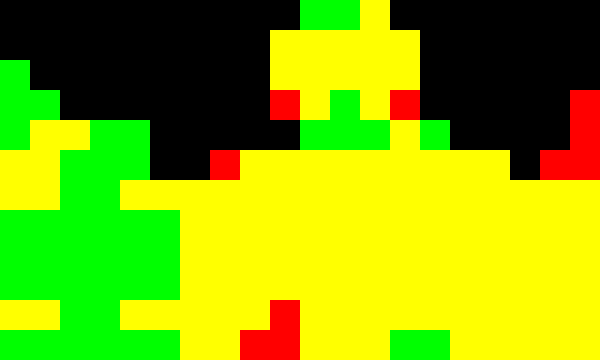
\includegraphics[scale=0.52]{img/cm.png}
    \caption{Material ID Range\cite{IGN}.}
    \label{fig:mir}
\end{figure}

\par At this point, \textit{Nanite} finally joins visibility and material together. The objective of the \textit{Visibility Buffer} is turning triangle information into surface properties. Unreal allows users to define arbitrary materials to surfaces, so how efficiently it manages that complexity? It uses an \textbf{Emit G-Buffer}.

\par That being said, \textit{Nanite} does one draw call per material ID, and every draw call is a full-screen quad chopped up into 240 squares rendered across the screen. As it was mentioned before, the material range texture is $240$ pixels, so every quad of this full-screen draw call has a corresponding texel\footnote{A texel is a term used in computer graphics to refer to a texture element.}. The quad vertices sample this texture and confirm whether the tile is a relevant tile; for example, whether any pixel in the tiles has the material corresponding to the material that's going to be rendered. If not, the $x$ coordinate will be set to $NaN$ and the whole quad is discarded.

\par According to the documentation, the system uses $14$ bits for \textit{Material IDs}, for a total of $16384$ maximum materials. A constant buffer sends the \textit{Material ID} to the vertex shader so that it can check whether it's in range.

\par Furthermore, it's necessary to remember that a material depth texture was created. This texture is where every \textit{Material ID} is set to be a certain depth. These quads are outputted to the depth represented by their material and the depth mode is set to equal, so the hardware can then very quickly discard any pixels that aren't relevant. As an extra step, the engine previously marks the stencil buffer as pixels that have \textit{Nanite Geometry} and regular pixels, also used for \textit{Early Z/Stencil} optimizations.

\begin{figure}[H]
    \centering
    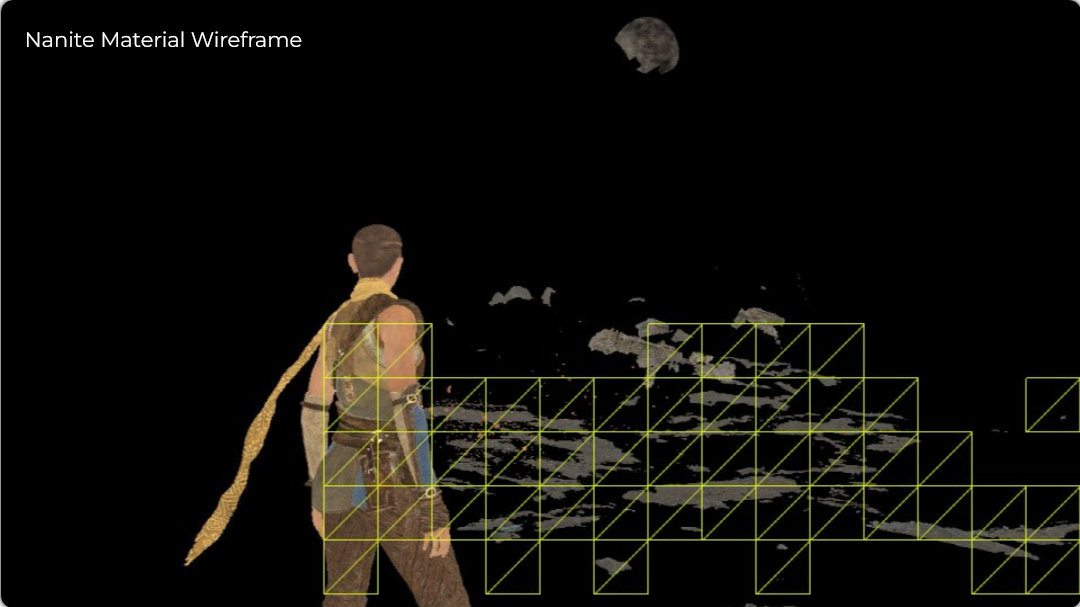
\includegraphics[scale=0.22]{img/wireframe.png}
    \caption{Nanite Material Wireframe\cite{IGN}.}
    \label{fig:wire}
\end{figure}

\begin{figure}[H]
    \centering
    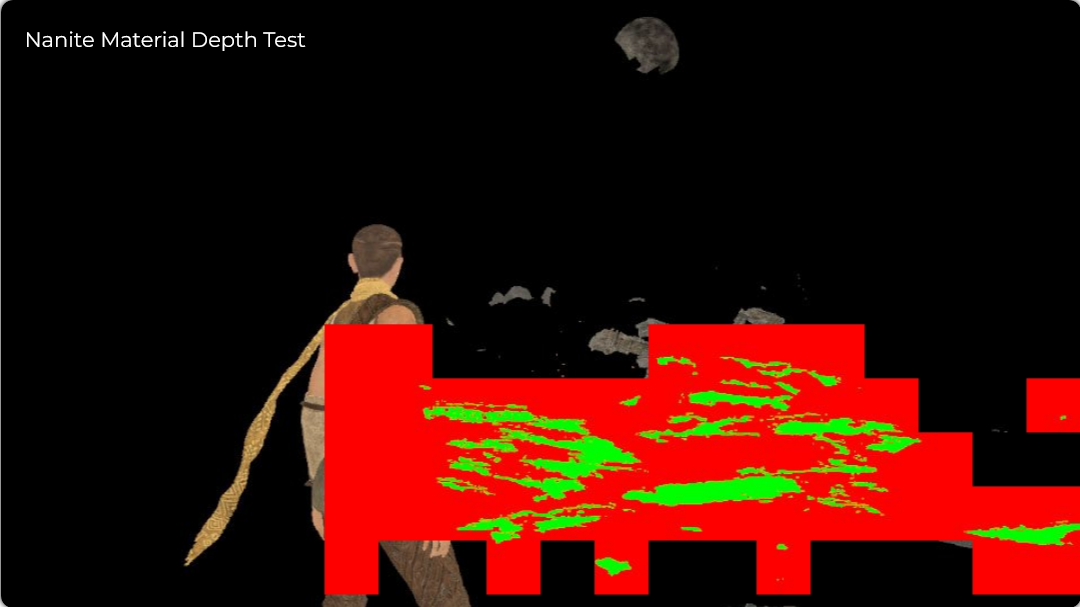
\includegraphics[scale=0.22]{img/Depth.png}
    \caption{Nanite Material Depth Test\cite{IGN}.}
    \label{fig:depth}
\end{figure}

\par As it can be noticed, some quads are completely red, which would lead to the conclusion that they are completely discarded by the vertex shader. However, it seems that the material range texture is exactly what it says: a range of materials covered by that tile. If a material happens to be “in the middle” but none of the pixels have it, it will be considered as a candidate even though the depth test will discard it completely later. In any case, that's the main idea – the same process as shown in the images is repeated until all materials are processed. The final \textit{G-Buffer} is show as tiles in the image below.

\begin{figure}[H]
    \centering
    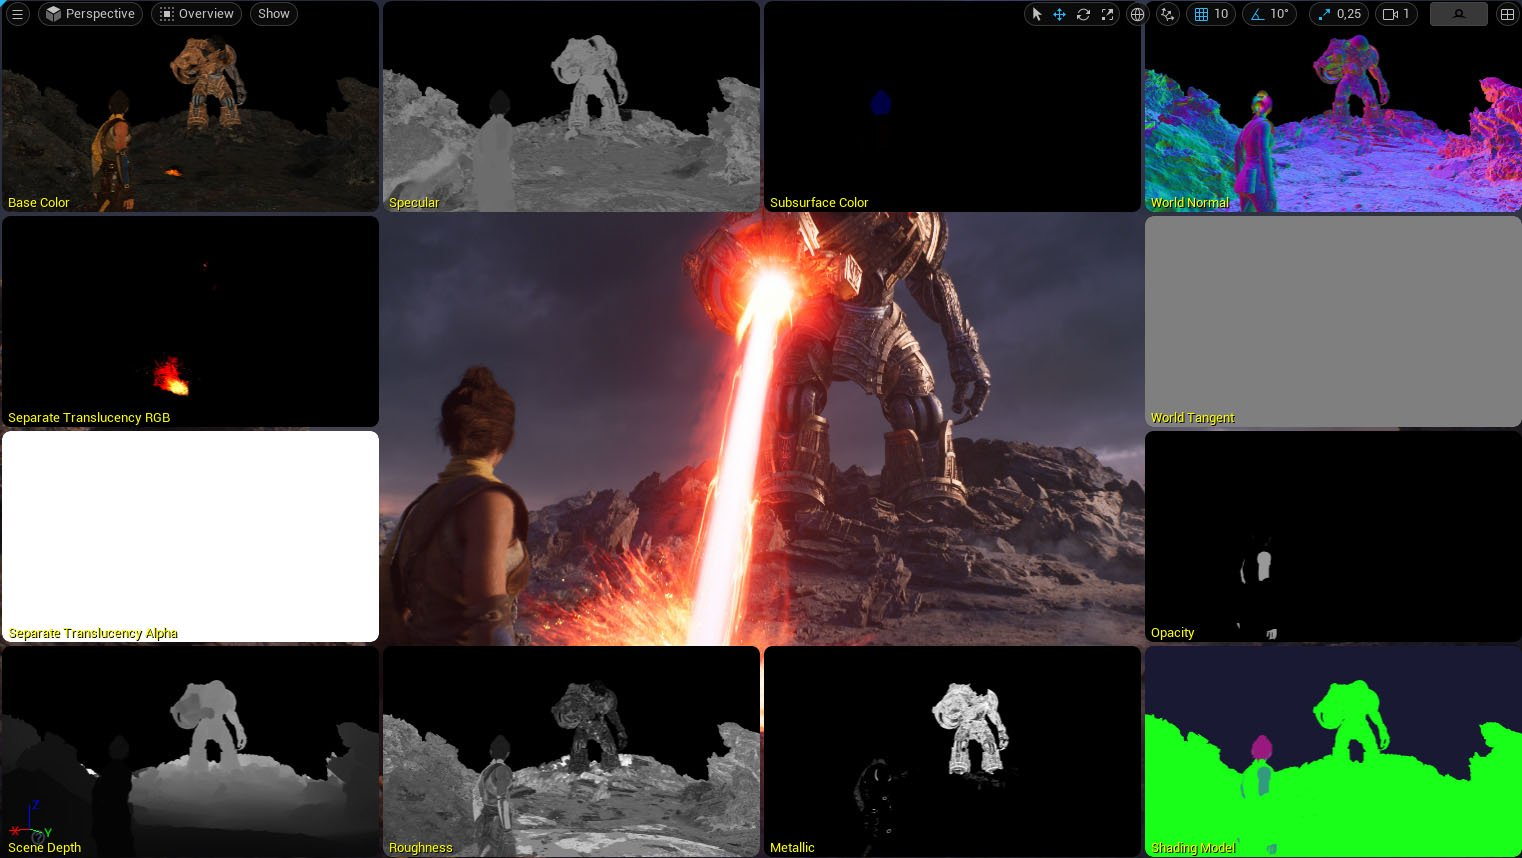
\includegraphics[scale=0.16]{img/fullBuff.jpg}
    \caption{\textit{G-Buffer} shown as tiles\cite{IGN}.}
    \label{fig:gbuff}
\end{figure}



%%%%%%%%%%%%%%%%%%%%%%%%%%%%%%%%%%%%%%%%%%%%%%%%%%%%%%%%%%%
%%%%%%%%%%%%%%%%%%%%%%%%%%%%%%%%%%%%%%%%%%%%%%%%%%%%%%%%%%%
\newpage
\section{The Power of Nanite}\label{sec:4}

\par In this section, we will explore some features of Unreal Engine's Nanite. By leveraging the power of virtualized textures and advanced algorithms, \textit{Nanite} allows developers to create highly detailed and realistic environments without worrying about the limitations of traditional polygon-based approaches. Let us delve into the key features of this cutting-edge technology and discover how it allows developers to achieve unprecedented levels of visual fidelity and immersion.

\subsection{Basic features}

\par \underline{\textbf{Geometry}}: in terms of geometry, \textit{Nanite} can be enabled on Static Meshes and Geometry Collections\footnote{Data structure and system used for handling and simulating complex physics interactions involving multiple pieces of geometry.}. Furthermore, a \textit{Nanite}-enable mesh can be used with the following Component types:
    \begin{itemize}
        \item Static Mesh 
        \item Instanced Static Mesh
        \item Hierarchical Instanced Static Mesh
        \item Geometry Collection
    \end{itemize}
    
\par One of the limitations \textit{Nanite} has in regard to geometry is that it can only be used on rigid meshes. Basically it can't be used on animated models like playable characters but works great on static objects that are often representative of a larger sample of geometry present in a scene.

\par \underline{\textbf{Materials}}: in regard to this matter, \textit{Nanite} is only capable of supporting Blend Mode set to \texttt{Opaque}. In computer graphics and image editing, blend modes are used to determine how pixels of one layer or object are combined with the pixels of another layer or background. When it comes to opaque materials, the blend mode typically used is \texttt{Normal}\footnote{Usually, the normal mode, or the default mode, replaces the pixels of the underlying layer with the pixels of the top layer, without any blending or transparency effects therefore it stays opaque.} or \texttt{Normal(Blend)}.

% \par When working with opaque materials, such as solid objects or surfaces, usually \textit{Nanite} tackles in a scene that doesn't have any transparency or translucency. Using the \texttt{Normal} blend mode ensures that the layer being blended appears solid and obscures any layers beneath it. It essentially ignores the \textit{alpha} channel or any transparency values associated with the layer.

\subsection{Hierarchical Dynamic Level of Detail - LODs}

\par Traditionally, renderers use techniques like pre-determined levels-of-detail\footnote{A good example is the different levels of subdivision when making the model. Each subdivision has a level of detail different from others.} and prebaked textures to optimize performance and manage memory, usually artists are heavily involved in this process. However, these methods often involve compromises in visual fidelity or require significant manual effort.

\par In \textit{Nanite}, \textbf{LOD}s are instead determined at a sub-mesh level, with much less artist involvement. That being said, \textit{Nanite}, instead of relying on pre-defined LOD meshes and textures, it allows the rendering of virtualized micropolygons.

\par So, a whole tree, or a directed acyclic graph (\textbf{DAG}), of $128$-triangle clusters is computed for each mesh at asset import time. The tree has $<= 128$ triangles  per node and the children of each node give a more in-depth look at that node. Then a “cut” of this tree is determined at runtime on the GPU and based on this “cut” a set of triangle clusters will be rendered. Culling also happens on a per-cluster, not per-mesh, basis.

\begin{figure}[H]
    \centering
    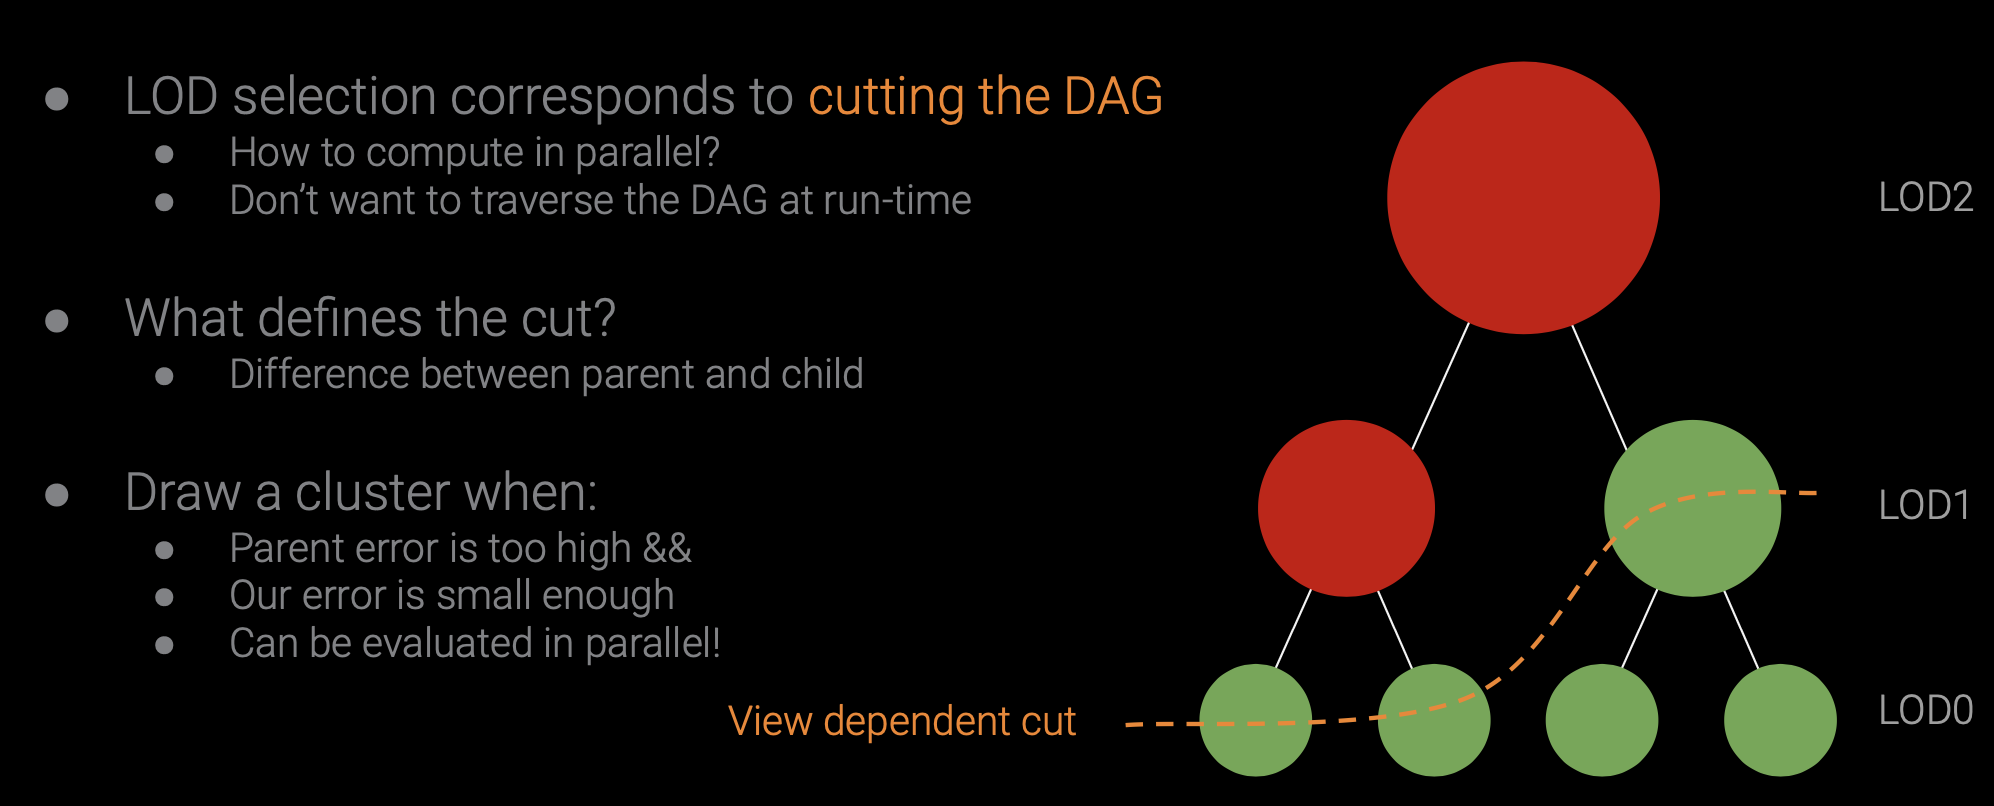
\includegraphics[scale=0.22]{img/VWe2y.png}
    \caption{Hierarchical Level of Detail\cite{karies_stubbe_wihlidal}}
    \label{fig:LODS}
\end{figure}

\par When all this comes together well,  a system with a very consistent number of triangles rendered to the screen per-frame and very little overdraw, also known as wasted shader work, is achieved. This efficiency is what lets \textit{Nanite} achieve high detail at decent \texttt{FPS} counts.

\par If not planned ahead, there might be problems with gaps between clusters, especially when they are next to each other in \textit{LOD} level $>1$. There might also exist visual popping when switching between \textit{LOD} levels. It is also possible to have problems with memory since there is a massive amount of data (each mesh has many tree clusters) and it needs a lot of GPU work to pre-shade them. 
\par With this, how does this cluster-based visibility culling happen on a GPU?

\subsubsection{Mesh simplification and hierarchy construction}

\par Firstly, a ton of work went into determining how triangles should be clustered and hierarchically arranged at asset-import-time so that cracks can't be observed, and yet it's still possible to efficiently determine a cut of this hierarchy at runtime. This involves complex graph partitioning and multidimensional optimization. 

\par It is also worth pointing out that the most detailed view of a mesh in \textit{Nanite}: the leaf nodes in the cluster graph are exactly the same triangles present in the original asset; \textit{Nanite} isn't capable of optimizing away detail, instead it displays simplified triangle clusters, higher nodes, only when the detail change isn't visually perceptible.

\subsubsection{LOD N vs LOD N+1}

\par One of the most novel contributions of \textit{Nanite} is the calculation of good perceptual error metrics between \textit{LODs}. Basically, it is needed to have the knowledge of how much worse a simpler triangle cluster is than its child (i.e. more detailed) clusters in order to do good \textit{LOD} selection. Amazingly, if the error difference is $<1$ pixel and some type of temporal antialiasing is present, there won't be any popping noticeable to the naked eye.

\subsubsection{Cutting the cluster hierarchy DAG (LOD Selection)}

\par A good cluster hierarchy and \textit{LOD} error calculations come together at runtime with view-based information\footnote{In GPU compute, using a bounding volume hierarchy (BVH) and custom parallel task system.} to determine the “cut” of the cluster \textit{DAG}, which is the \textit{LOD} selection of that frame.

% \subsection{Cluster-based visibility culling}

% \par For visibility culling, a modified “two-pass occlusion culling”\cite{niebner_loop} technique is used. In this technique, it is used what's visible in a previous frame\footnote{Captured in a hierarchical z-buffer (HZB).} to massively speed up the determination of what's visible in the frame. \textit{Nanite} diverges somewhat from other two-pass culling systems because they use a bunch of information from the \textit{LOD} selection phase described above to make this work. The output of this visibility check is then written to a “visibility buffer” that includes pre-pixel depth and cluster index data.

%\subsubsection{Material selection and shading}

%\par Once the visibility data is obtained, material shading is needed, which outputs to g-buffers\footnote{Intermediate rendering buffer that stores multiple types of information about a scene or objects within a scene.} and the rest of deferred shading pipeline. That being said, the material shading per pixels works as follows:

%\begin{enumerate}
%    \item Load VisBuffer
%    \item Load instance transform
%    \item Load 3 vert indexes
%    \item Load 3 positions
%    \item Transform positions to screen
%    \item Derive barycentric coordinates for pixel
%    \item Load and lerp attributes
%\end{enumerate}

%\par This workflow can achieve a good cache hit-rate and almost no overdraw\cite{karies_stubbe_wihlidal_3}.

\subsection{Fallback Mesh}

\par When \textit{Nanite} is enabled for a Static Mesh, it creates a simplified version of the intricate mesh that can be accessed and utilized in situations where \textit{Nanite} data is not applicable. This simplified mesh, known as the \textbf{Fallback Mesh}, serves as a substitute when \textit{Nanite} rendering is not supported. It is particularly useful in scenarios where it is impractical to use the high-detail mesh, such as when complex collision detection is necessary, for example.

\begin{figure}[H]
    \centering
    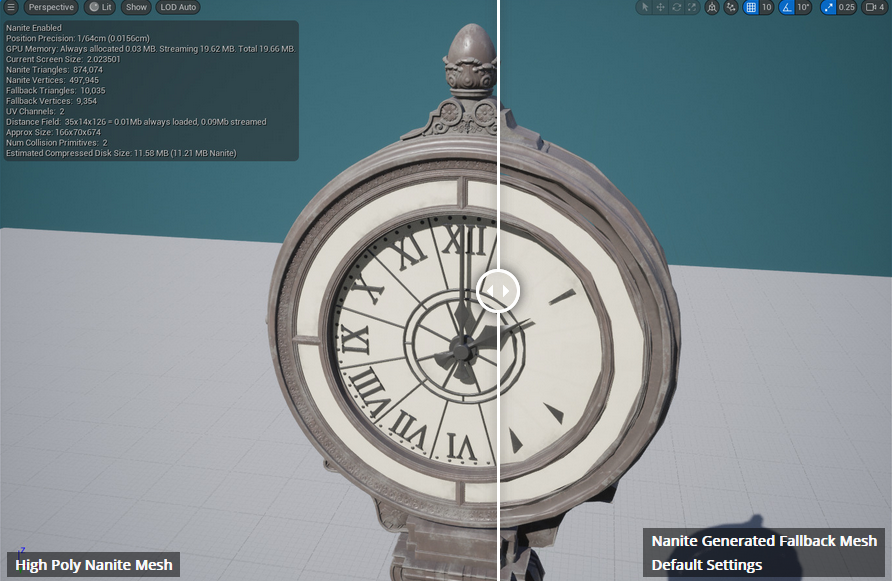
\includegraphics[scale=0.37]{img/fallback.png}
    \caption{\textit{Nanite} Generated Fallback Mesh\cite{Unreal}.}
    \label{fig:Fallback}
\end{figure}

\par It's worth noting that there is the possibility of adjusting values like the \textbf{Fallback Relative Error} to specify how much of the original detail is retained from the original source mesh, and Fallback Percentage to set how much of that detail is used.

\begin{figure}[H]
    \centering
    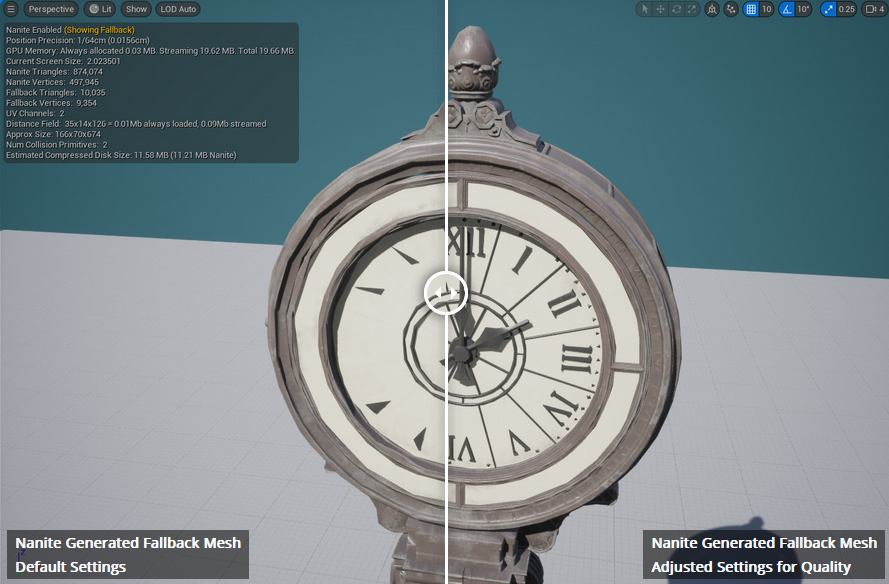
\includegraphics[scale=0.37]{img/fallback2.png}
    \caption{Fallback Mesh with default settings vs adjusted settings\cite{Unreal}.}
    \label{fig:Fallback2}
\end{figure}

\subsection{Streaming virtual geometry}

\par For memory management, \textit{Nanite} aggressively ejects unused clusters from working memory and stream in new ones from disk. For this reason, a decent SSD is basically required for \textit{Nanite} to work. This is what's called “virtual geometry”, analogous to “virtual texturing”. Formatting, compressing and deciding what to stream is complex. About approximately 1M input asset triangles become almost $11 Mb$ compressed \textit{Nanite} data on disk\cite{karies_stubbe_wihlidal_2}.

%%%%%%%%%%%%%%%%%%%%%%%%%%%%%%%%%%%%%%%%%%%%%%%%%%%%%%%%%%%
%%%%%%%%%%%%%%%%%%%%%%%%%%%%%%%%%%%%%%%%%%%%%%%%%%%%%%%%%%%

\section{Experimentation}\label{sec:5}

\par After this extensive analysis on the technology, it's worth seeing it in action. With this, some test scenarios were developed in order to show the true power of \textit{Nanite}.

\par Firstly, all tests were made on a machine with the following specifications:

\begin{itemize}
    \item \textbf{CPU:} AMD Ryzen 7 5800H with Radeon Graphics 3.20 GHz
    \item \textbf{RAM:} 32.0 GB (31.4 GB usable)
    \item \textbf{GPU:} NVIDIA GeForce RTX 3080 Laptop GPU
\end{itemize}

\par With the help of UE5, a new empty scene was created with the Unreal Started Content contained in it. After creating a new landscape using the mode \texttt{Landscape}, in order to place any object on the scene, it was chosen the following model as the test model.

\begin{figure}[H]
    \centering
    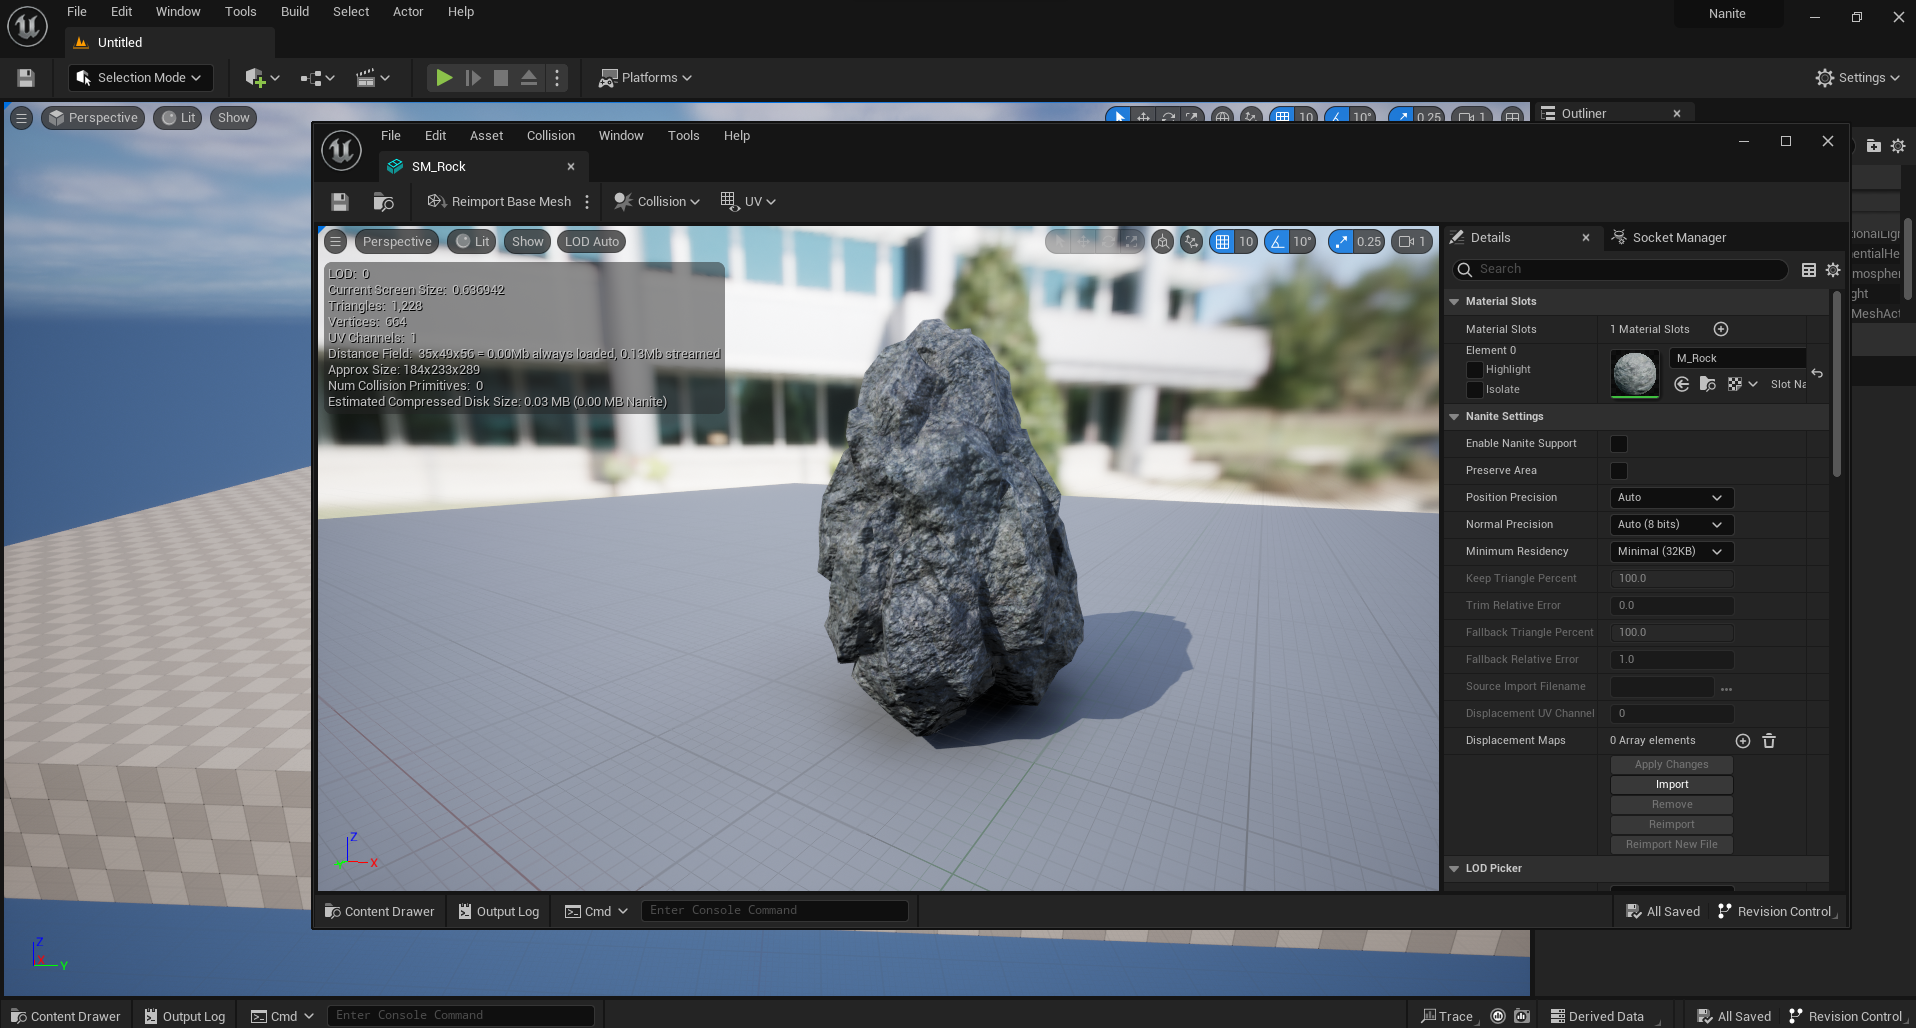
\includegraphics[scale=0.16]{img/rock.png}
    \caption{Test\_1 Model – Starter Content Rock.}
    \label{fig:rock}
\end{figure}

\par After this, the mode \texttt{Foliage} was used to place numerous instances of the same model onto the landscape. With this, the testing scene contained \textbf{160k instances} of the chosen mesh for the tests. It's also worth mentioning that the command \texttt{Stats fps} was used in order to check the fps count of the scene and comparing results. \underline{Without \textit{Nanite}}, the scene obtained a fps count of \textbf{20.64 fps}. So, it can be seen that, even the machine being fairly powerful,  the number of instances reduces greatly the frames per second of this scene.

\par To solve this problem, \textit{Nanite} was enabled and applied to the test mesh. This will apply \textit{Nanite} to all the instances of the mesh that are present in the terrain. To check if \textit{Nanite} was enabled properly, it was inspected if one of the information textures that \textit{Nanite} creates was present.

\begin{figure}[H]
    \centering
    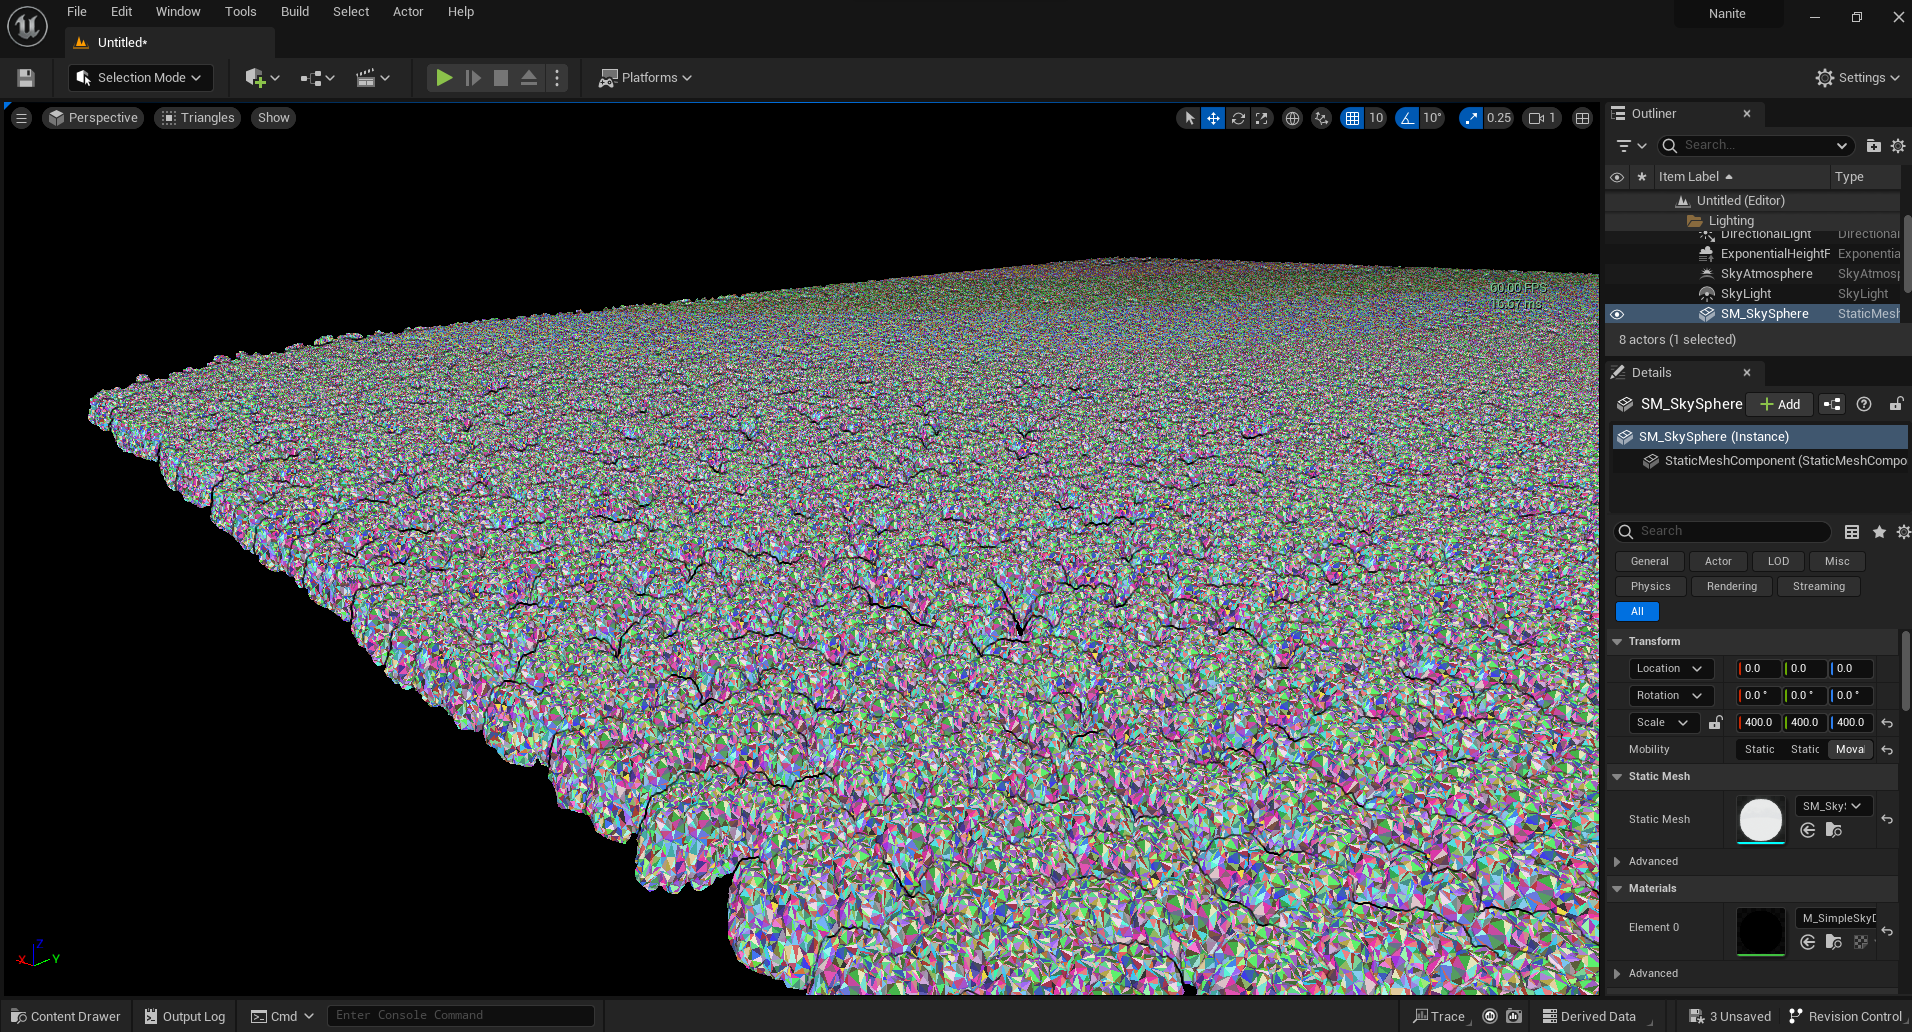
\includegraphics[scale=0.16]{img/naniterocks.png}
    \caption{Test\_1 Triangle ID texture is present, confirming that \textit{Nanite} was enabled properly.}
    \label{fig:tidrock}
\end{figure}

\par Now, with \underline{\textit{Nanite} enabled}, the scene achieves an astounding fps count of \textbf{60 fps} (possibly capped by UE5 system definitions).

\par To further prove that \textit{Nanite} can do what it sets out to do, a second Test scenario was made. This time it was used a third party static mesh in order to prove that \textit{Nanite} works on external meshes and not just the ones made available by Epic Games.

\begin{figure}[H]
    \centering
    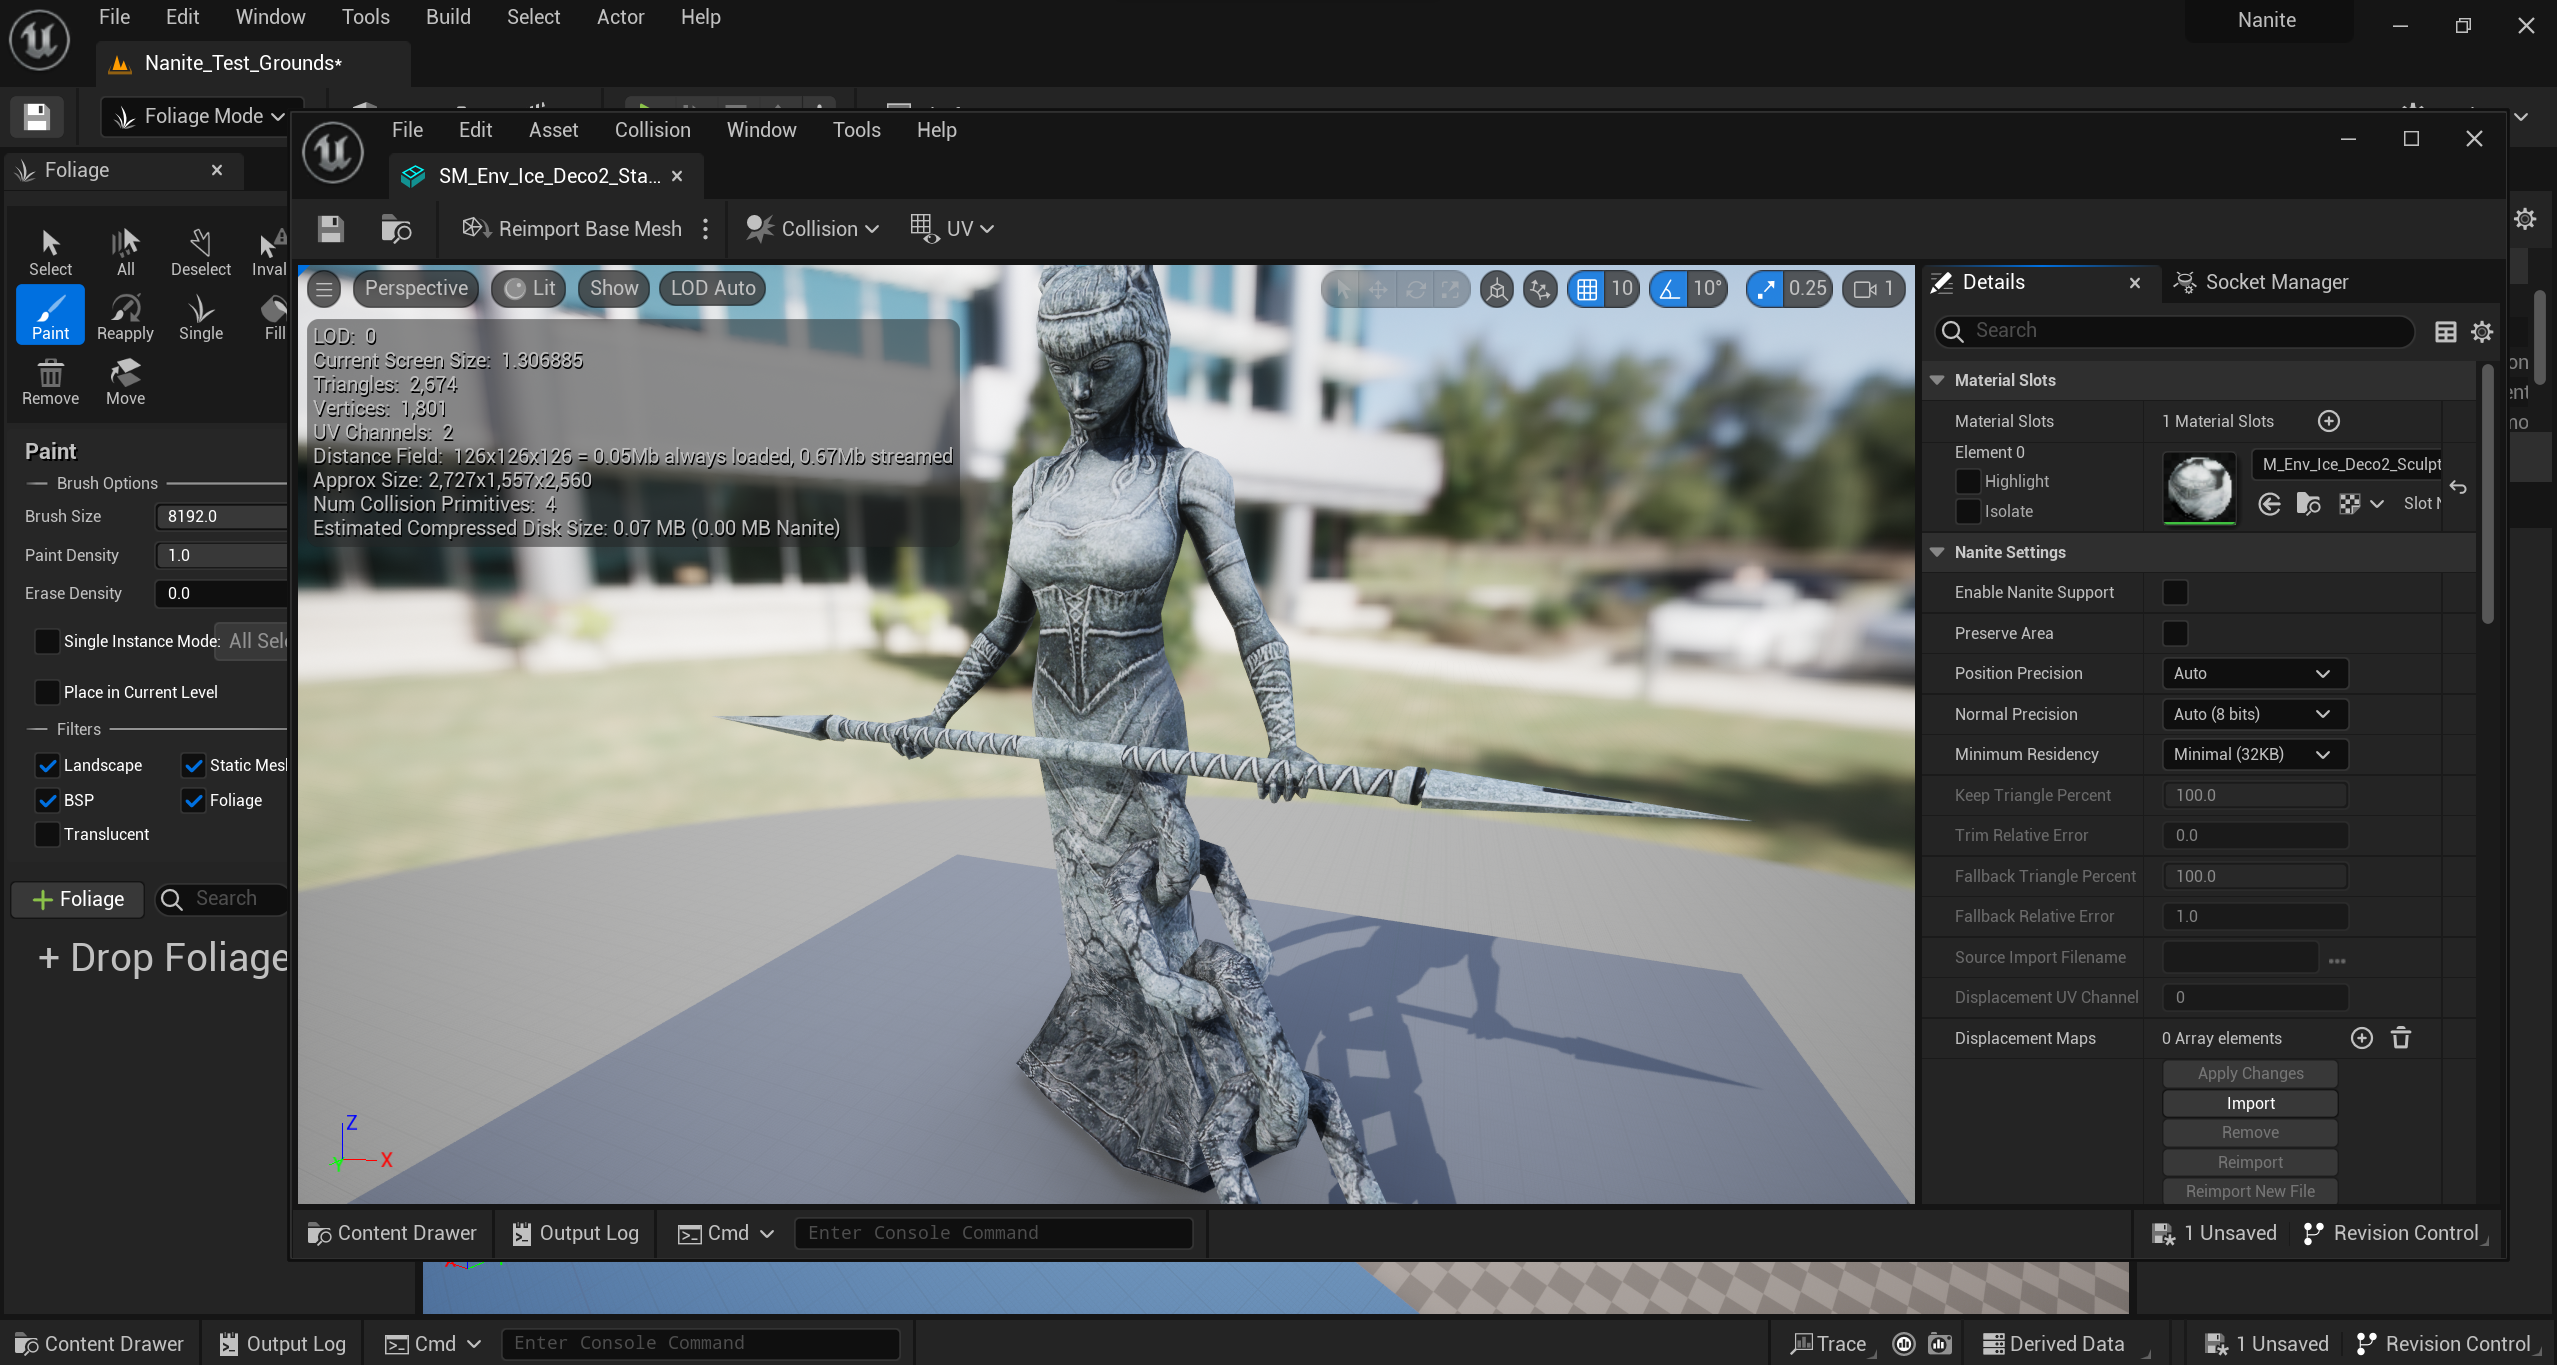
\includegraphics[scale=0.16]{img/image.png}
    \caption{Test\_2 Model – Infinity Blade: Ice Lands Statue.}
    \label{fig:statue}
\end{figure}

\begin{figure}[H]
    \centering
    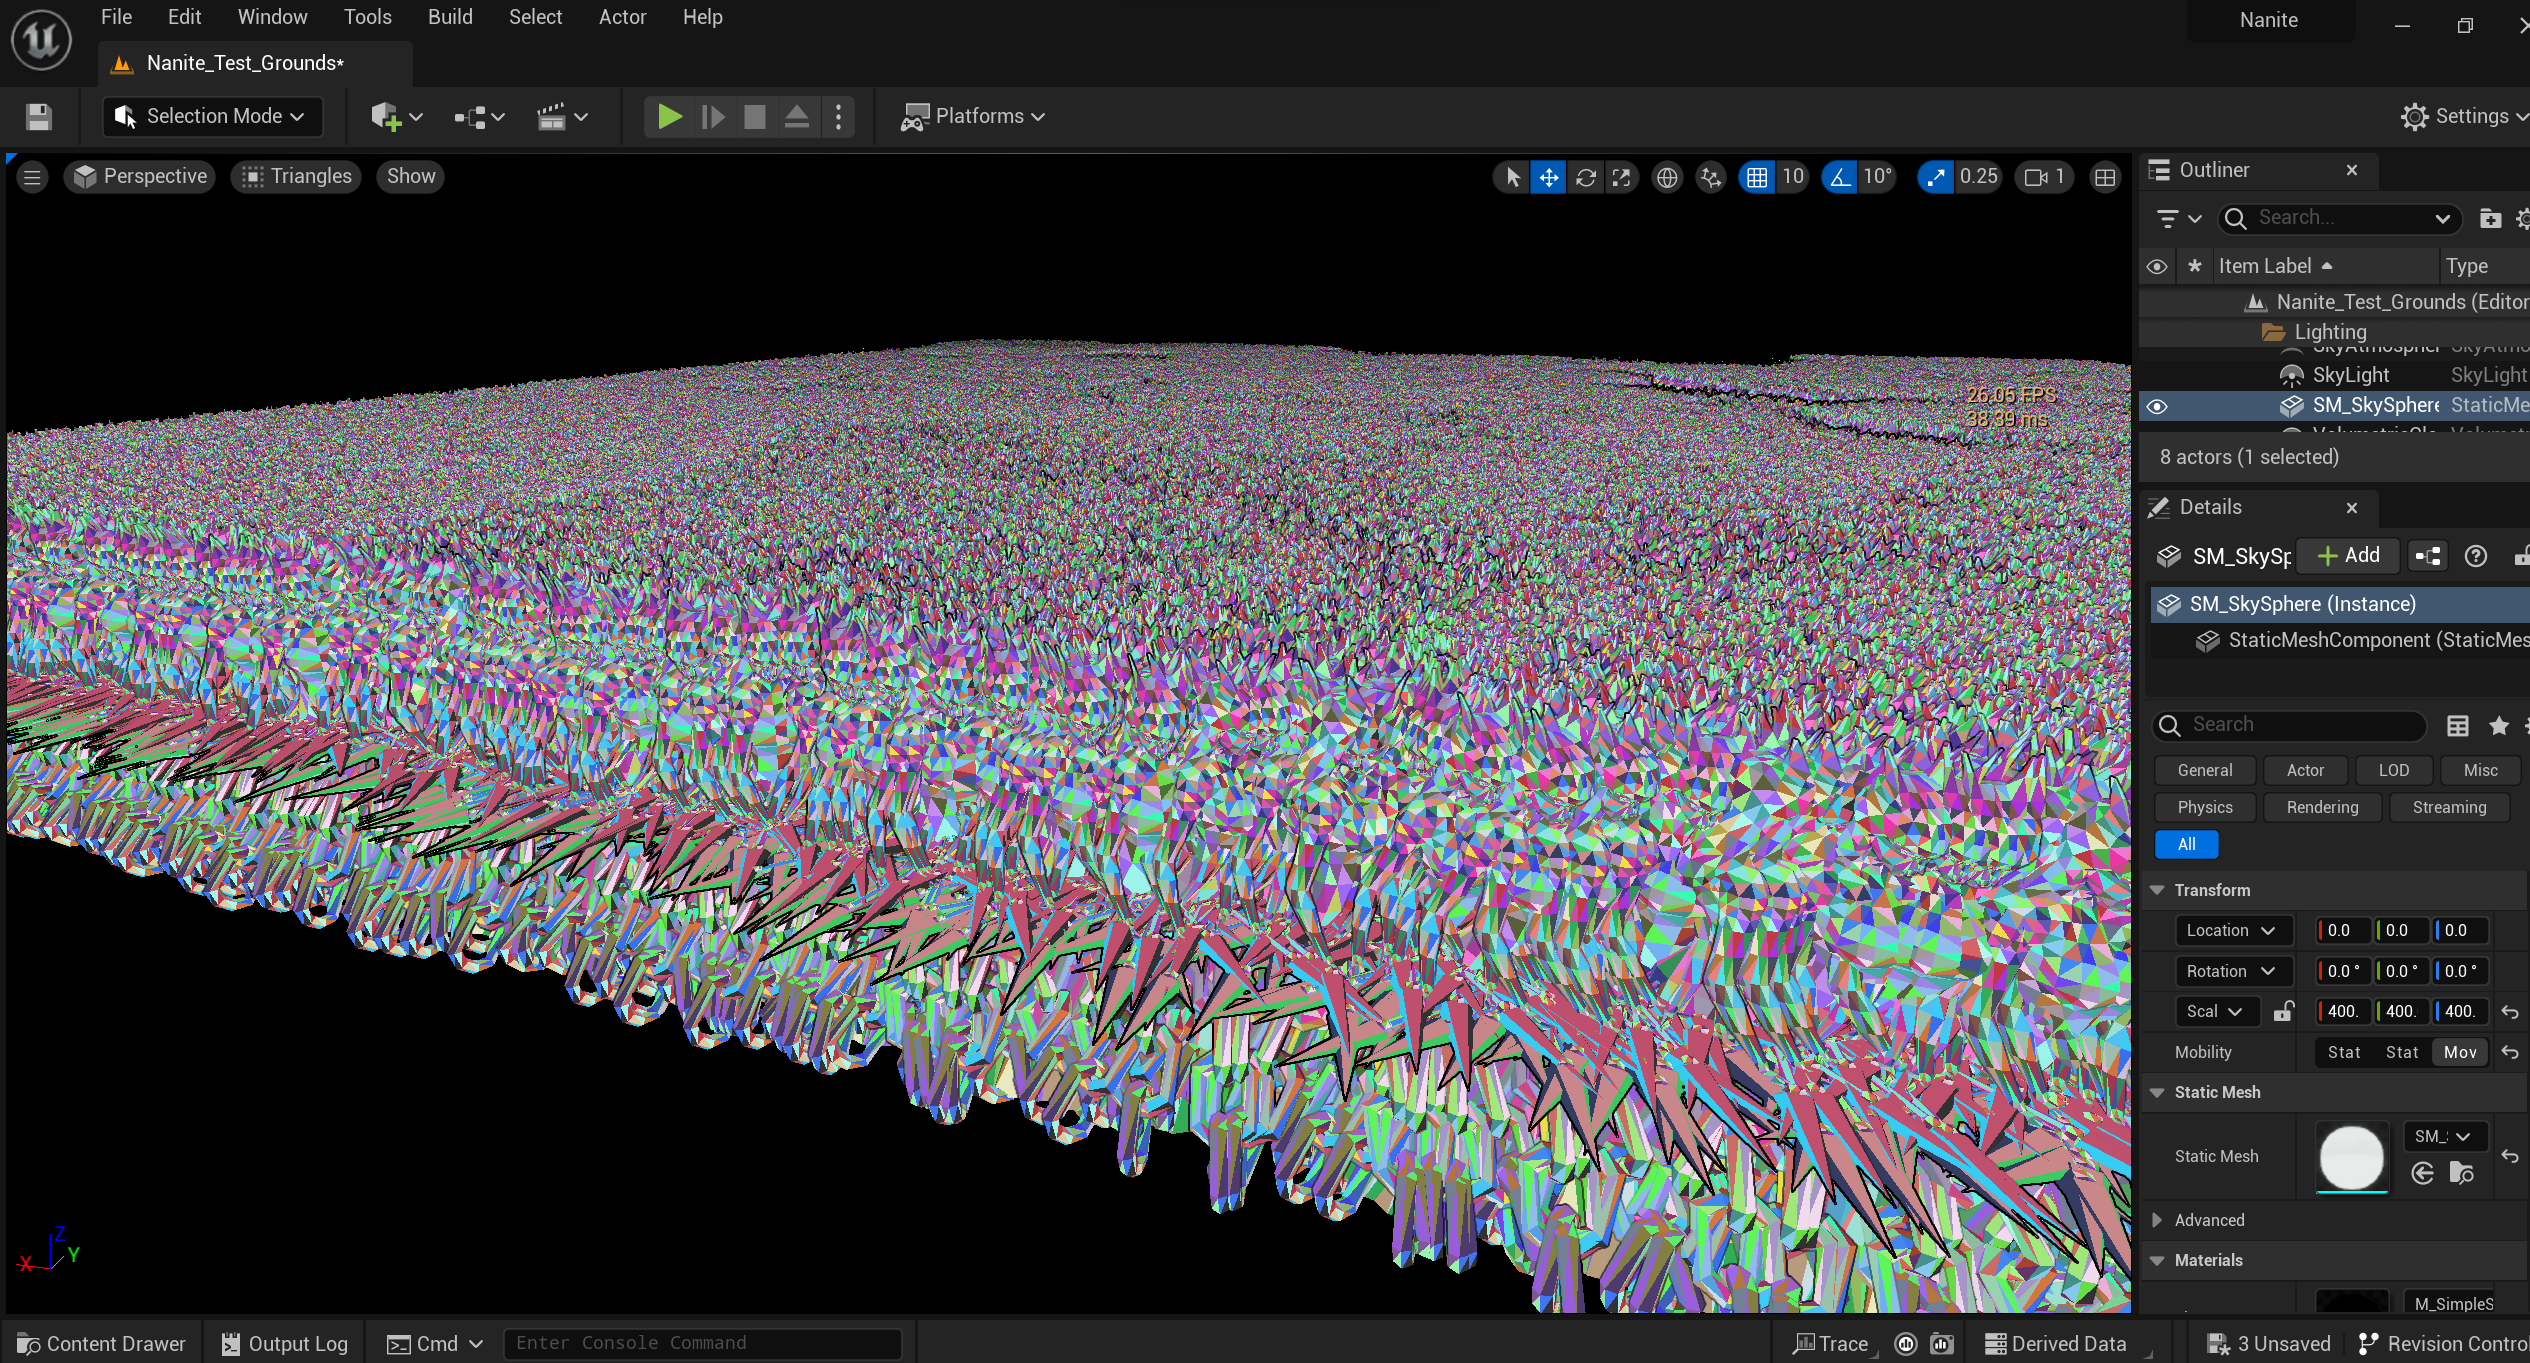
\includegraphics[scale=0.16]{img/image2.png}
    \caption{Test\_2 Triangle ID texture is present, confirming that \textit{Nanite} was enabled properly.}
    \label{fig:tidstatue}
\end{figure}

\par In this test scenario, the geometry of the mesh is much more detailed than the previous one. With this, \underline{without \textit{Nanite}}, it can only achieve \textbf{14.56 fps}, having an instance count of $89.5k$. \underline{With \textit{Nanite}}, it achieves a fps count of \textbf{58.20 fps}.

\par This confirms that \textit{Nanite} can indeed improve the performance of a scene with numerous static meshes contained in it. To further illustrate this enhancement in performance, the subsequent graph is presented.

\begin{figure}[H]
    \centering
    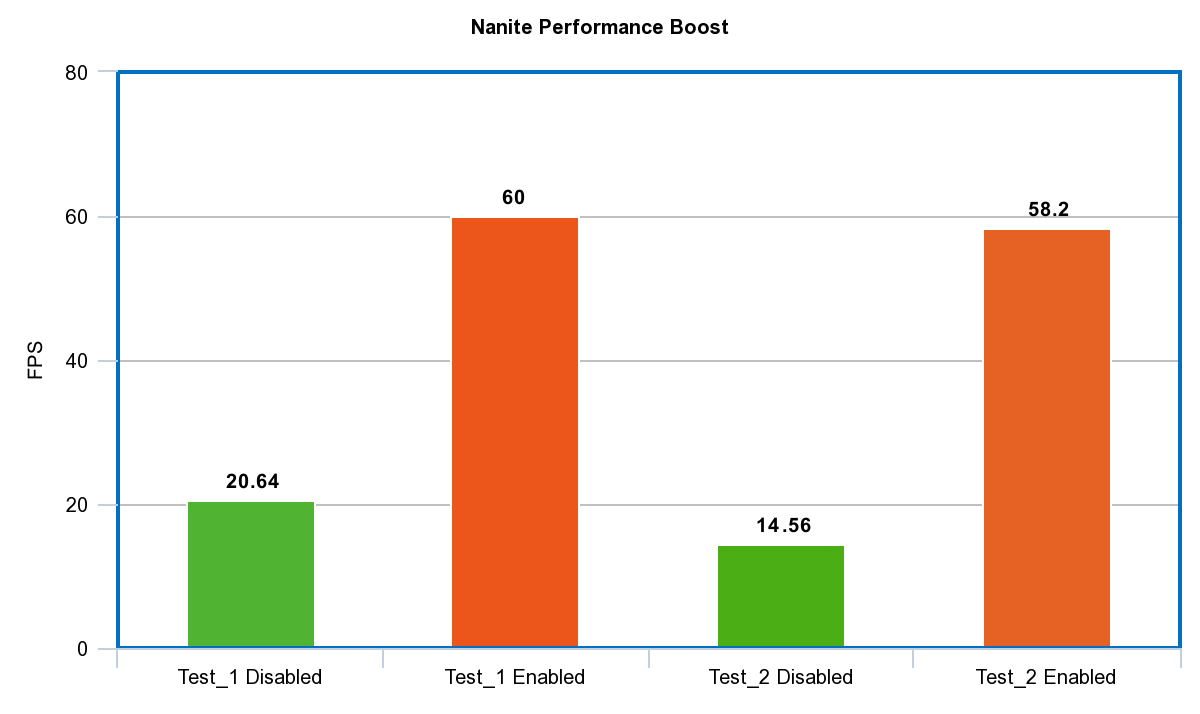
\includegraphics[scale=0.2]{img/meta-chart.png}
    \caption{\textit{Nanite} performance comparison.}
    \label{fig:stats}
\end{figure}

%%%%%%%%%%%%%%%%%%%%%%%%%%%%%%%%%%%%%%%%%%%%%%%%%%%%%%%%%%%
%%%%%%%%%%%%%%%%%%%%%%%%%%%%%%%%%%%%%%%%%%%%%%%%%%%%%%%%%%%

\section{Conclusions}\label{sec:7}

\par \textit{Unreal Engine's Nanite} represents a significant advancement in real-time rendering technology, pushing the boundaries of what is possible in terms of visual fidelity and scalability. By introducing virtualized micropolygon geometry, \textit{Nanite} eliminates the limitations of traditional rasterization techniques, allowing for the rendering of highly detailed scenes with unprecedented levels of geometry complexity. This breakthrough technology not only revolutionizes the way developers create and optimize assets, but also offers a new level of immersion and realism for players.

\par The state-of-the-art nature of \textit{Nanite} is evident in its ability to render massive scenes without sacrificing performance or compromising on visual quality. Leveraging the power of virtualized micropolygons and material streaming, \textit{Nanite} provides an efficient solution for rendering geometry-rich environments, making it an invaluable tool for game developers, filmmakers, and other industries that require high-fidelity rendering.

\par The implementation of \textit{Nanite} showcases the remarkable engineering and design efforts undertaken by Epic Games. The integration of virtualized micropolygon geometry into the existing Unreal Engine ecosystem demonstrates a thoughtful and comprehensive approach to delivering cutting-edge technology to developers. \textit{Nanite}'s seamless integration with other features such as \textit{Lumen}, the dynamic global illumination system, further enhances its capabilities and opens up new possibilities for creating visually stunning experiences.

\par While \textit{Nanite} undoubtedly represents a breakthrough in real-time rendering technology, there are still areas for further exploration and refinement. As the technology evolves, addressing potential challenges such as memory management and optimizing performance for a broader range of hardware configurations will be crucial. Additionally, continued research and development efforts can expand \textit{Nanite}'s potential applications beyond gaming, into fields such as architectural visualization, virtual reality, and simulations.

\par In conclusion, \textit{Unreal Engine's Nanite} is a groundbreaking technology that redefines the state of the art in real-time rendering. With its ability to handle massive scenes and deliver unprecedented levels of detail, \textit{Nanite} empowers developers to create immersive and visually stunning experiences. As the technology continues to advance, it can be expected \textit{Nanite} to play an increasingly significant role in shaping the future of real-time graphics.

\newpage
\bibliographystyle{IEEEtran}
\bibliography{cp}
\end{document}